\documentclass[12pt]{book}
\usepackage[utf8]{inputenc}
\usepackage[T1]{fontenc}
\usepackage[paperwidth=6in, paperheight=9in, margin=0.75in]{geometry}
\usepackage{amsmath}
\usepackage{lmodern}
\usepackage{enumitem}
\usepackage{pgfplots}
\pgfplotsset{compat=1.15}
\usepackage{mathrsfs}
\usetikzlibrary{arrows}
\usepackage{float}
\usepackage{wrapfig} % Pour enrouler le texte autour des images
\usepackage{graphicx} % Pour inclure des images
\usepackage{microtype} % Amélioration typographique
\usepackage[table]{xcolor} % Pour une meilleure gestion des couleurs
\usepackage{array}
\usepackage{bm}

\renewcommand{\arraystretch}{2.5}
		
%\let\cleardoublepage\clearpage



\usepackage{fancyhdr}
\usepackage[french]{babel}

\usepackage[colorlinks=true, linkcolor=blue]{hyperref}
\usepackage{xurl} % Casse les URLs longues proprement
\usepackage{cleveref} % Pour les références intelligentes
\usepackage{etoolbox}

\makeatletter
\newcommand{\urllist}{}
\newcounter{urlcounter}

% Commande principale simplifiée
\newcommand{\urlnote}[2]{%
    \refstepcounter{urlcounter}%
    \label{urlpage:\theurlcounter}% Label standard
    \href{#2}{#1}\footnote{\url{#2}}%
    \protected@xappto{\urllist}{%
        \noexpand\item[#1] \noexpand\url{#2}%
        \noexpand\space(voir page~\noexpand\pageref{urlpage:\theurlcounter})%
    }%
}

% Affichage de l'annexe
\newcommand{\printurlannexe}{%
    \chapter*{Annexe des URLs}
    \addcontentsline{toc}{chapter}{Annexe des URLs}
    \ifdefvoid{\urllist}
        {\textit{Aucun URL enregistré.}}
        {\begin{description}
            \urllist
        \end{description}}%
}
\makeatother


% Définition des couleurs
\definecolor{myblue}{RGB}{0,0,139}
\definecolor{mygreen}{RGB}{0,100,0}

% Configuration des listes
\setlist[enumerate]{itemsep=0.5em, topsep=0.5em}
\setlist[itemize]{itemsep=0.5em, topsep=0.5em}

% Amélioration de l'interligne
\linespread{1.1}

%\pagestyle{fancy}
%\fancyhf{}
%\rhead{\textcolor{myblue}{Calcul et géométrie}}
%\lhead{\textcolor{myblue}{\sc Laurent Garnier}}
%\rfoot{\thepage}

%\title{Exercices de calculs et représentations géométriques}
%\author{\textsc{Laurent Garnier}}
%\date{}

\begin{document}
\pagestyle{plain}                        % ↳ numéros en pied de page, en-têtes vides
%\maketitle

% ----------------- Page de titre (exemple sobre) -----------
\begin{titlepage}
    \centering
    %\Huge\bfseries Exercices de calculs et représentations géométriques\\[2cm]
    %\Large \textsc{Laurent Garnier}\\[1cm]
    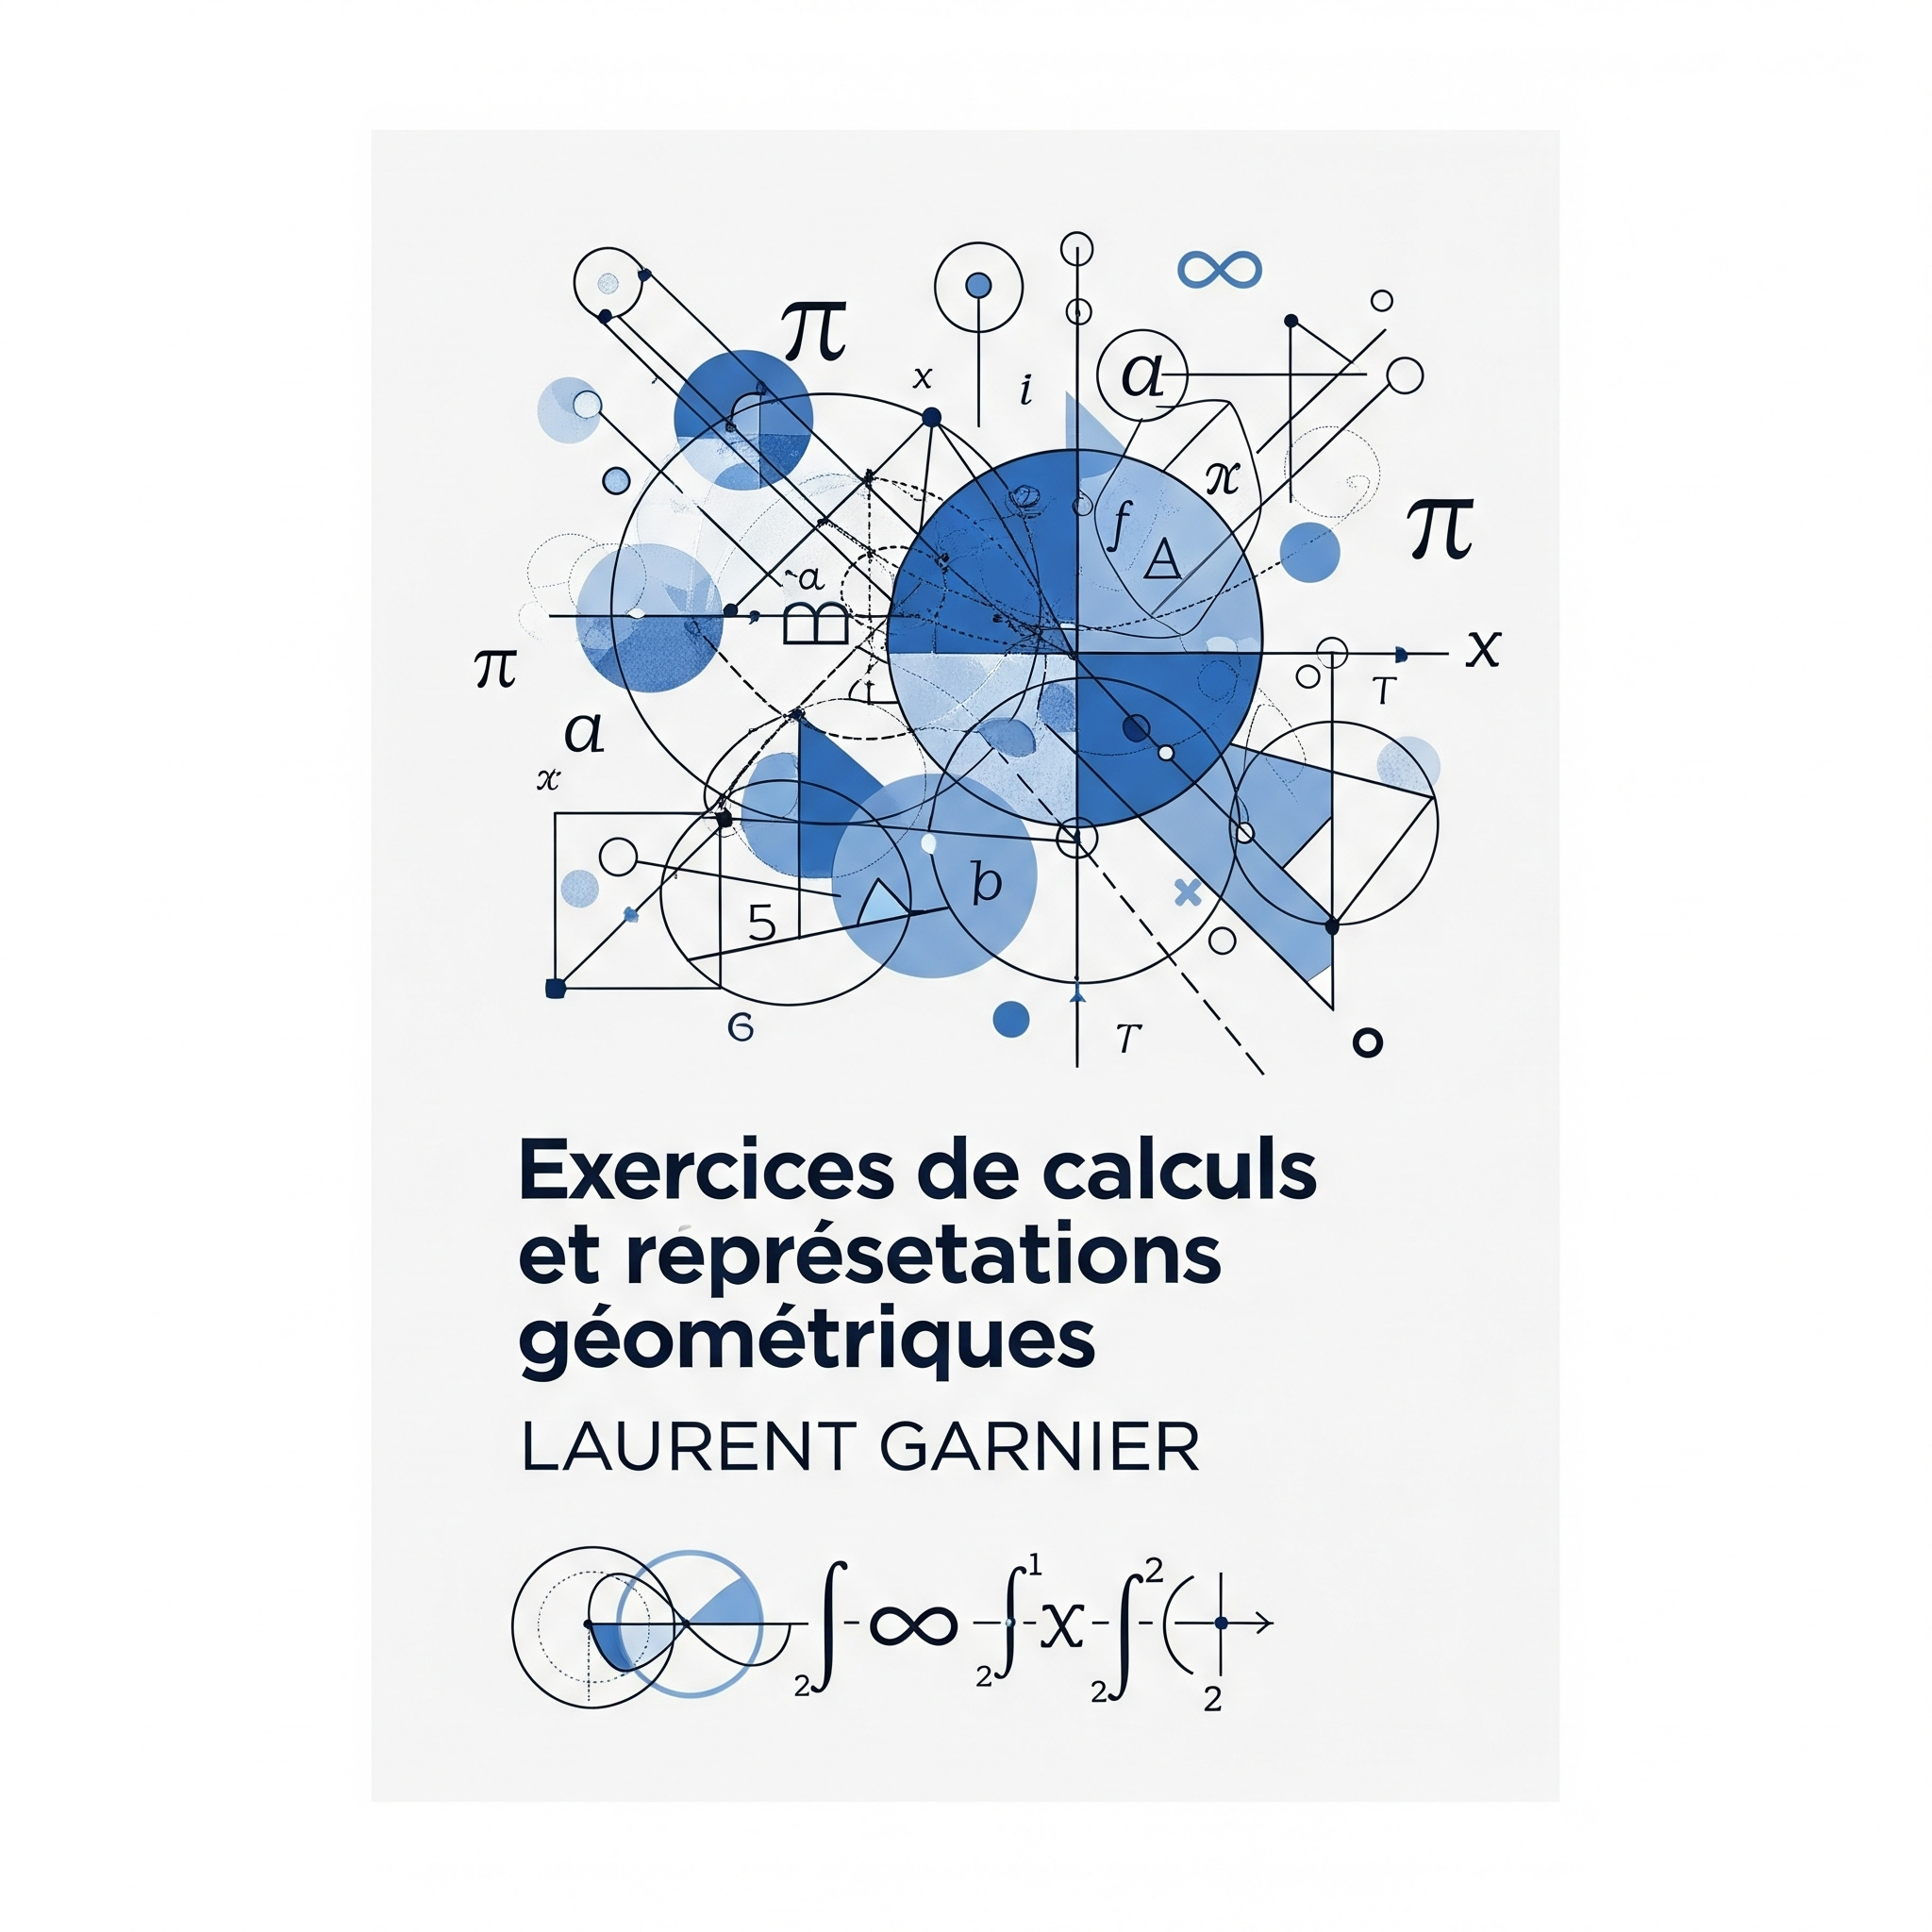
\includegraphics[width=1.0\textwidth]{../images/cover.png}\\[2cm]
    \normalsize \copyright\ 2025 \textsc{Laurent Garnier} – Tous droits réservés
\end{titlepage}
%\cleardoublepage

% ============  AVANT-PROPOS éventuel  ======================
\frontmatter      % numérotation romaine (i, ii, …) pour les pages préliminaires

% ----------------- SOMMAIRE NON DÉTAILLÉ -------------------
\chapter*{Sommaire succint}
\begin{itemize}
  \item \hyperlink{chap1}{\textbf{Un peu de culture historique}}
  \item \hyperlink{chap:level1}{\textbf{Niveau primaire}}
  \item \hyperlink{chap:level2}{\textbf{Niveau secondaire : collège}}
  \item \hyperlink{chap:level3}{\textbf{Niveau secondaire : lycée}}
  \item \hyperlink{chap:sol}{\textbf{Solutions des exercices}}
  \item \hyperlink{chap:and-now}{\textbf{Et maintenant ?}}
\end{itemize}
\cleardoublepage


% ============  CORPS DU LIVRE  =============================
\mainmatter       % passe en numérotation arabe (1, 2, …)

\hypertarget{chap1}{}
\chapter{Un peu de culture historique}\label{chap1}

\section{Introduction}
\addcontentsline{toc}{chapter}{Introduction}


Ce livre a pour but de vous faire faire des mathématiques. On commence par du calcul mental afin d’échauffer l’esprit. Oui, même au XXI\up{e} siècle, alors que nous avons des calculatrices, des ordinateurs, des téléphones et même des intelligences artificielles, il est encore utile d’exercer son cerveau sur ce genre de tâches. Loin de moi l’idée de vous prendre pour des calculateurs prodiges, ni d’essayer de vous entraîner à le devenir : je n’en suis pas un, et j’aurais du mal à vous aider pour ce genre de compétitions. Mais, de la même façon que les humains n’ont pas cessé de marcher et de courir après l’invention de la voiture, de l’ascenseur et des autres moyens de transport, il en va de même pour l’exercice cérébral. Sans être médecin, il me semble que le bon sens nous dicte que, si l’on reste assis sur le canapé à manger de la malbouffe sans faire de sport, il y a de gros risques de rencontrer des problèmes de surpoids et de santé en général. L’exercice cérébral est une gymnastique de l’esprit : c'est une \urlnote{hygiène mentale}{https://www.youtube.com/watch?v=qrA5HgFIjJE}.

Néanmoins, il serait vain — et surtout ennuyeux — de se cantonner aux calculs. L’activité mathématique est bien plus riche que cela. Il ne s’agit pas de comptabilité. Même si l’arithmétique et le calcul algébrique restent des outils cruciaux dans l’architecture des mathématiques, les maths ne se résument pas à des calculs. D’un autre côté, oublier cet aspect serait une carence aussi flagrante que celle d’un sportif de haut niveau (footballeur, nageur, judoka… choisissez votre sport favori) qui ne ferait pas de musculation. Les sportifs font de la musculation parce que leurs muscles sont leurs outils pour accomplir leur art. En mathématiques, c’est pareil : les calculs et la capacité à les conduire sont utiles pour résoudre des problèmes mathématiques.

Ce livre s’articule en trois parties principales, en plus de cette introduction.

La première partie doit être faite par tous les lecteurs en guise d’échauffement. Il s’agit de calculs \frquote{\textit{purs et durs}}, de niveau primaire. En effet, l’école primaire a pour but de faire acquérir la maîtrise des quatre opérations de l’arithmétique de base, à savoir : addition, soustraction, multiplication et division. Cela peut paraître simple, mais derrière ces \frquote{\textit{simples}} opérations se cachent les structures algébriques que nous aborderons dans un prochain ouvrage consacré à l’enseignement supérieur.

Dans la seconde partie, on passe au niveau collège, en ajoutant des calculs de carrés, des programmes de calculs, le calcul littéral, les liens entre géométrie et calcul, et des probabilités de base en termes de rapports d’aires de figures élémentaires.

Enfin, dans la troisième partie, on passe au niveau lycée : configurations de nombres, vecteurs, statistiques et situations concrètes. Mais les choses sont présentées avec un vocabulaire et des connaissances accessibles à un collégien. 

Le souhait de cet ouvrage est de fournir des exercices faisables directement, sans avoir à \textit{réviser le cours}. Trop souvent aujourd’hui, les élèves sont traumatisés par la crainte de ne pas connaître \frquote{\textit{la phrase du cours}}, comme s’il s’agissait d’une incantation magique. Aucun cours de mathématiques n’est tombé du ciel, telles les tables de la Loi. L’activité mathématique s’est développée au cours des siècles à travers des problèmes qui, une fois résolus, ont donné lieu à des généralisations, lesquelles sont ensuite devenues des cours. Alors bien sûr, on ne peut pas se permettre le luxe de tout redémontrer à partir de zéro, sinon chaque génération aurait à refaire tout ce qu’a fait la précédente. Néanmoins, il me semble beaucoup plus intéressant, et surtout utile et efficace, de s’exercer d’abord ; et, à force de pratique, le cours pourra alors être vu comme quelque chose d’intéressant… un nouveau genre d’exercice.

Ma critique première est que les enseignements primaires et secondaires (surtout primaire et collège) manquent cruellement de démonstrations (alors que des démonstrations géométriques sont accessibles très tôt comme par exemple la \urlnote{démonstration de la 1\up{ère} identité remarquable}{https://youtu.be/IL55ftyJQHI} ), au profit d’un apprentissage par cœur dénué de raisonnement et de réflexion, destiné à créer des \frquote{\textit{automatismes}}. À l’époque de l’intelligence artificielle, il me semble d’autant plus absurde de vouloir former des générations d’automates, déjà dépassés par les véritables automates. Nous, humains, faisons des erreurs et avons la capacité d’apprendre de nos erreurs. C’est précisément pour cette raison qu’il faut cultiver l’art de se tromper intelligemment.

L’art de se tromper intelligemment signifie prendre le risque de pousser un raisonnement jusqu’à son terme, pour se rendre compte s’il fonctionne ou non. Comprendre signifie prendre un risque : sans prise de risque, vous ne pourrez jamais comprendre ; sans erreur, vous ne pourrez jamais comprendre.

Ici, tous les exercices sont corrigés, donc vous pouvez les faire en toute honnêteté, en prenant véritablement le risque de vous tromper. De plus, pour la plupart des exercices (en dehors de ceux de calculs purs), il y a souvent plusieurs façons de les résoudre. Il ne faut donc pas chercher à mémoriser les corrections. Les exercices sont presque tous originaux ou des adaptations de classiques.

\newpage

Pour toutes remarques, suggestions, ou demandes d'aide personnelles merci de remplir \urlnote{ce formulaire}{https://forms.gle/x7fAce7GqiJAGbsC7} : \url{https://forms.gle/x7fAce7GqiJAGbsC7}. Si vous souhaitez obtenir la version numérique de ce livre c'est aussi ce même formulaire qu'il faut remplir afin que nous puissions entrer en contact.

\newpage 

\subsection{Origine étymologique du mot calcul}

\begin{wrapfigure}[5]{l}{0.4\textwidth} % 8 = lignes occupées, l = à gauche
    \vspace{-0.75cm} % remonte l’image pour l’aligner avec la 1ère ligne du texte
    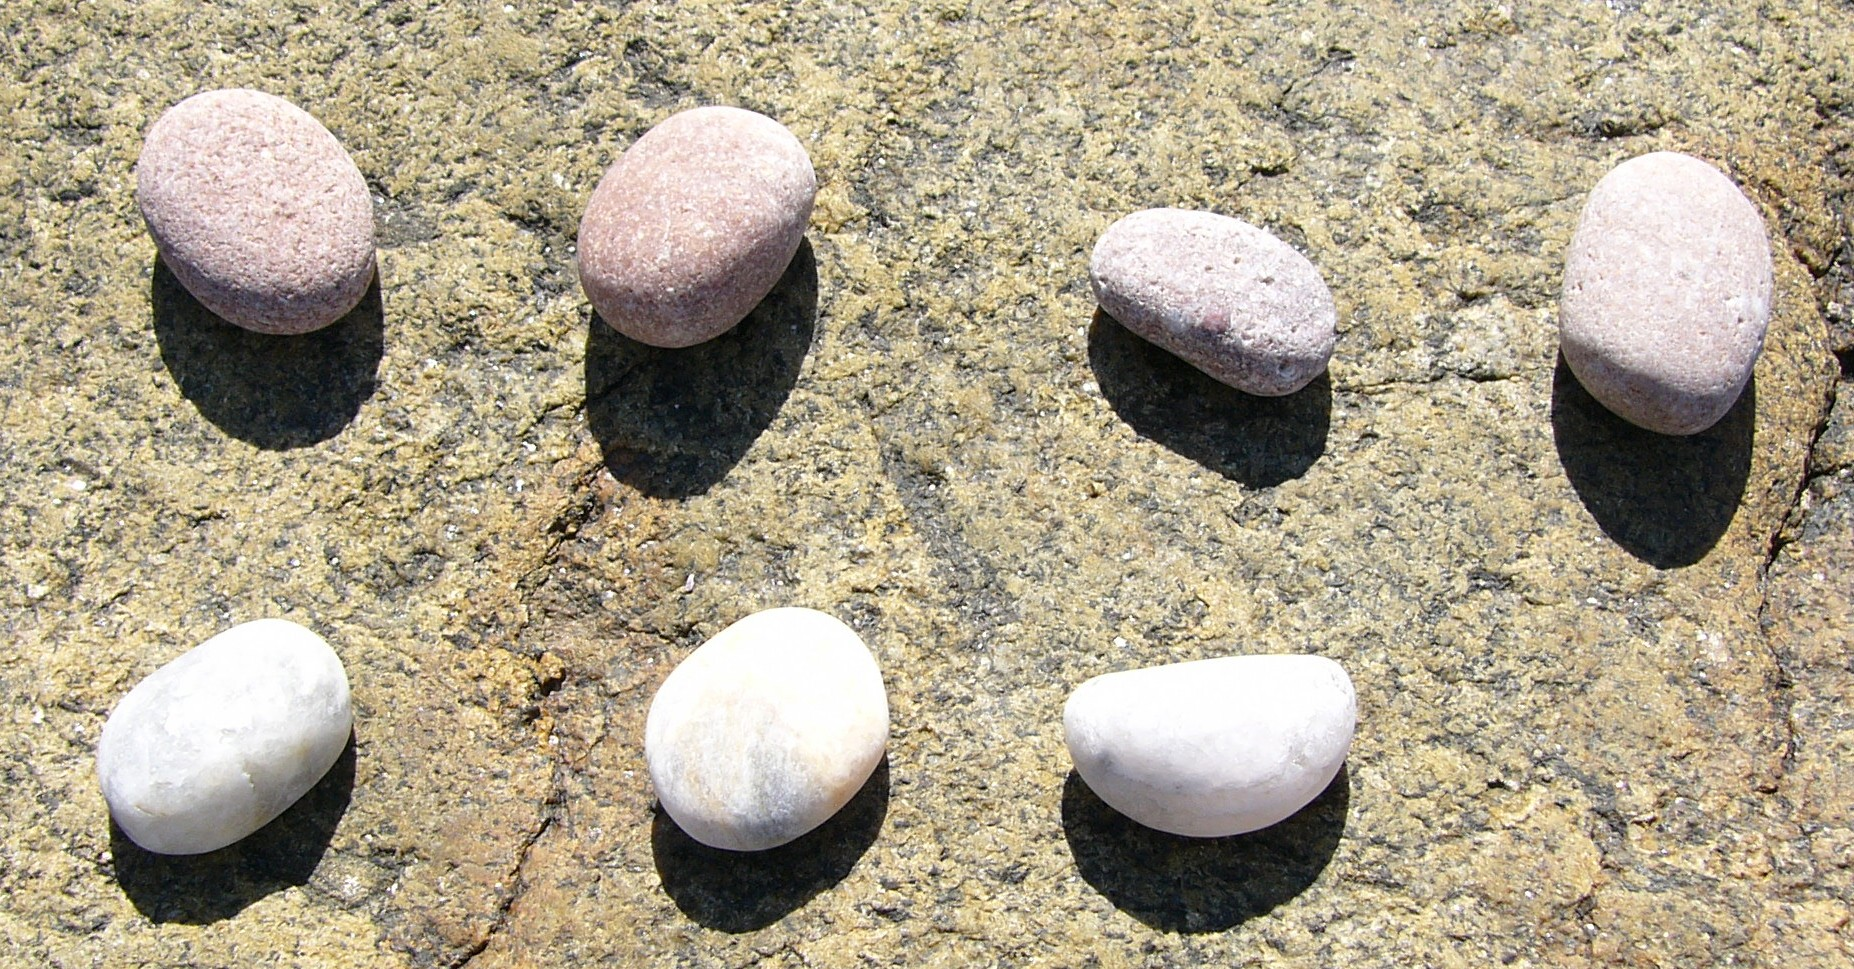
\includegraphics[width=0.4\textwidth]{../images/Cailloux.jpeg}
    %\caption{}
\end{wrapfigure}

Le mot \frquote{calcul} vient du latin \textbf{\textit{calculus}}, qui signifiait littéralement \frquote{petit caillou}. Ce terme dérive de \textbf{\textit{calx}}, \textbf{\textit{calcis}} (chaux, pierre calcaire). Les Romains utilisaient effectivement de petits cailloux ou jetons pour effectuer leurs opérations arithmétiques sur l'abaque, d'où cette étymologie concrète qui reflète une pratique réelle. 

\newpage 

\subsection{Premières traces de calculs}

Les plus anciennes traces de calculs remontent à la préhistoire :

\vspace{.5cm}



\textsc{Os d'Ishango} (République démocratique du Congo, ~20 000 ans) : 

\vspace{.2cm}

\begin{wrapfigure}[8]{l}{0.22\textwidth} % 8 = lignes occupées, l = à gauche
    \vspace{-0.65cm} % remonte l’image pour l’aligner avec la 1ère ligne du texte
    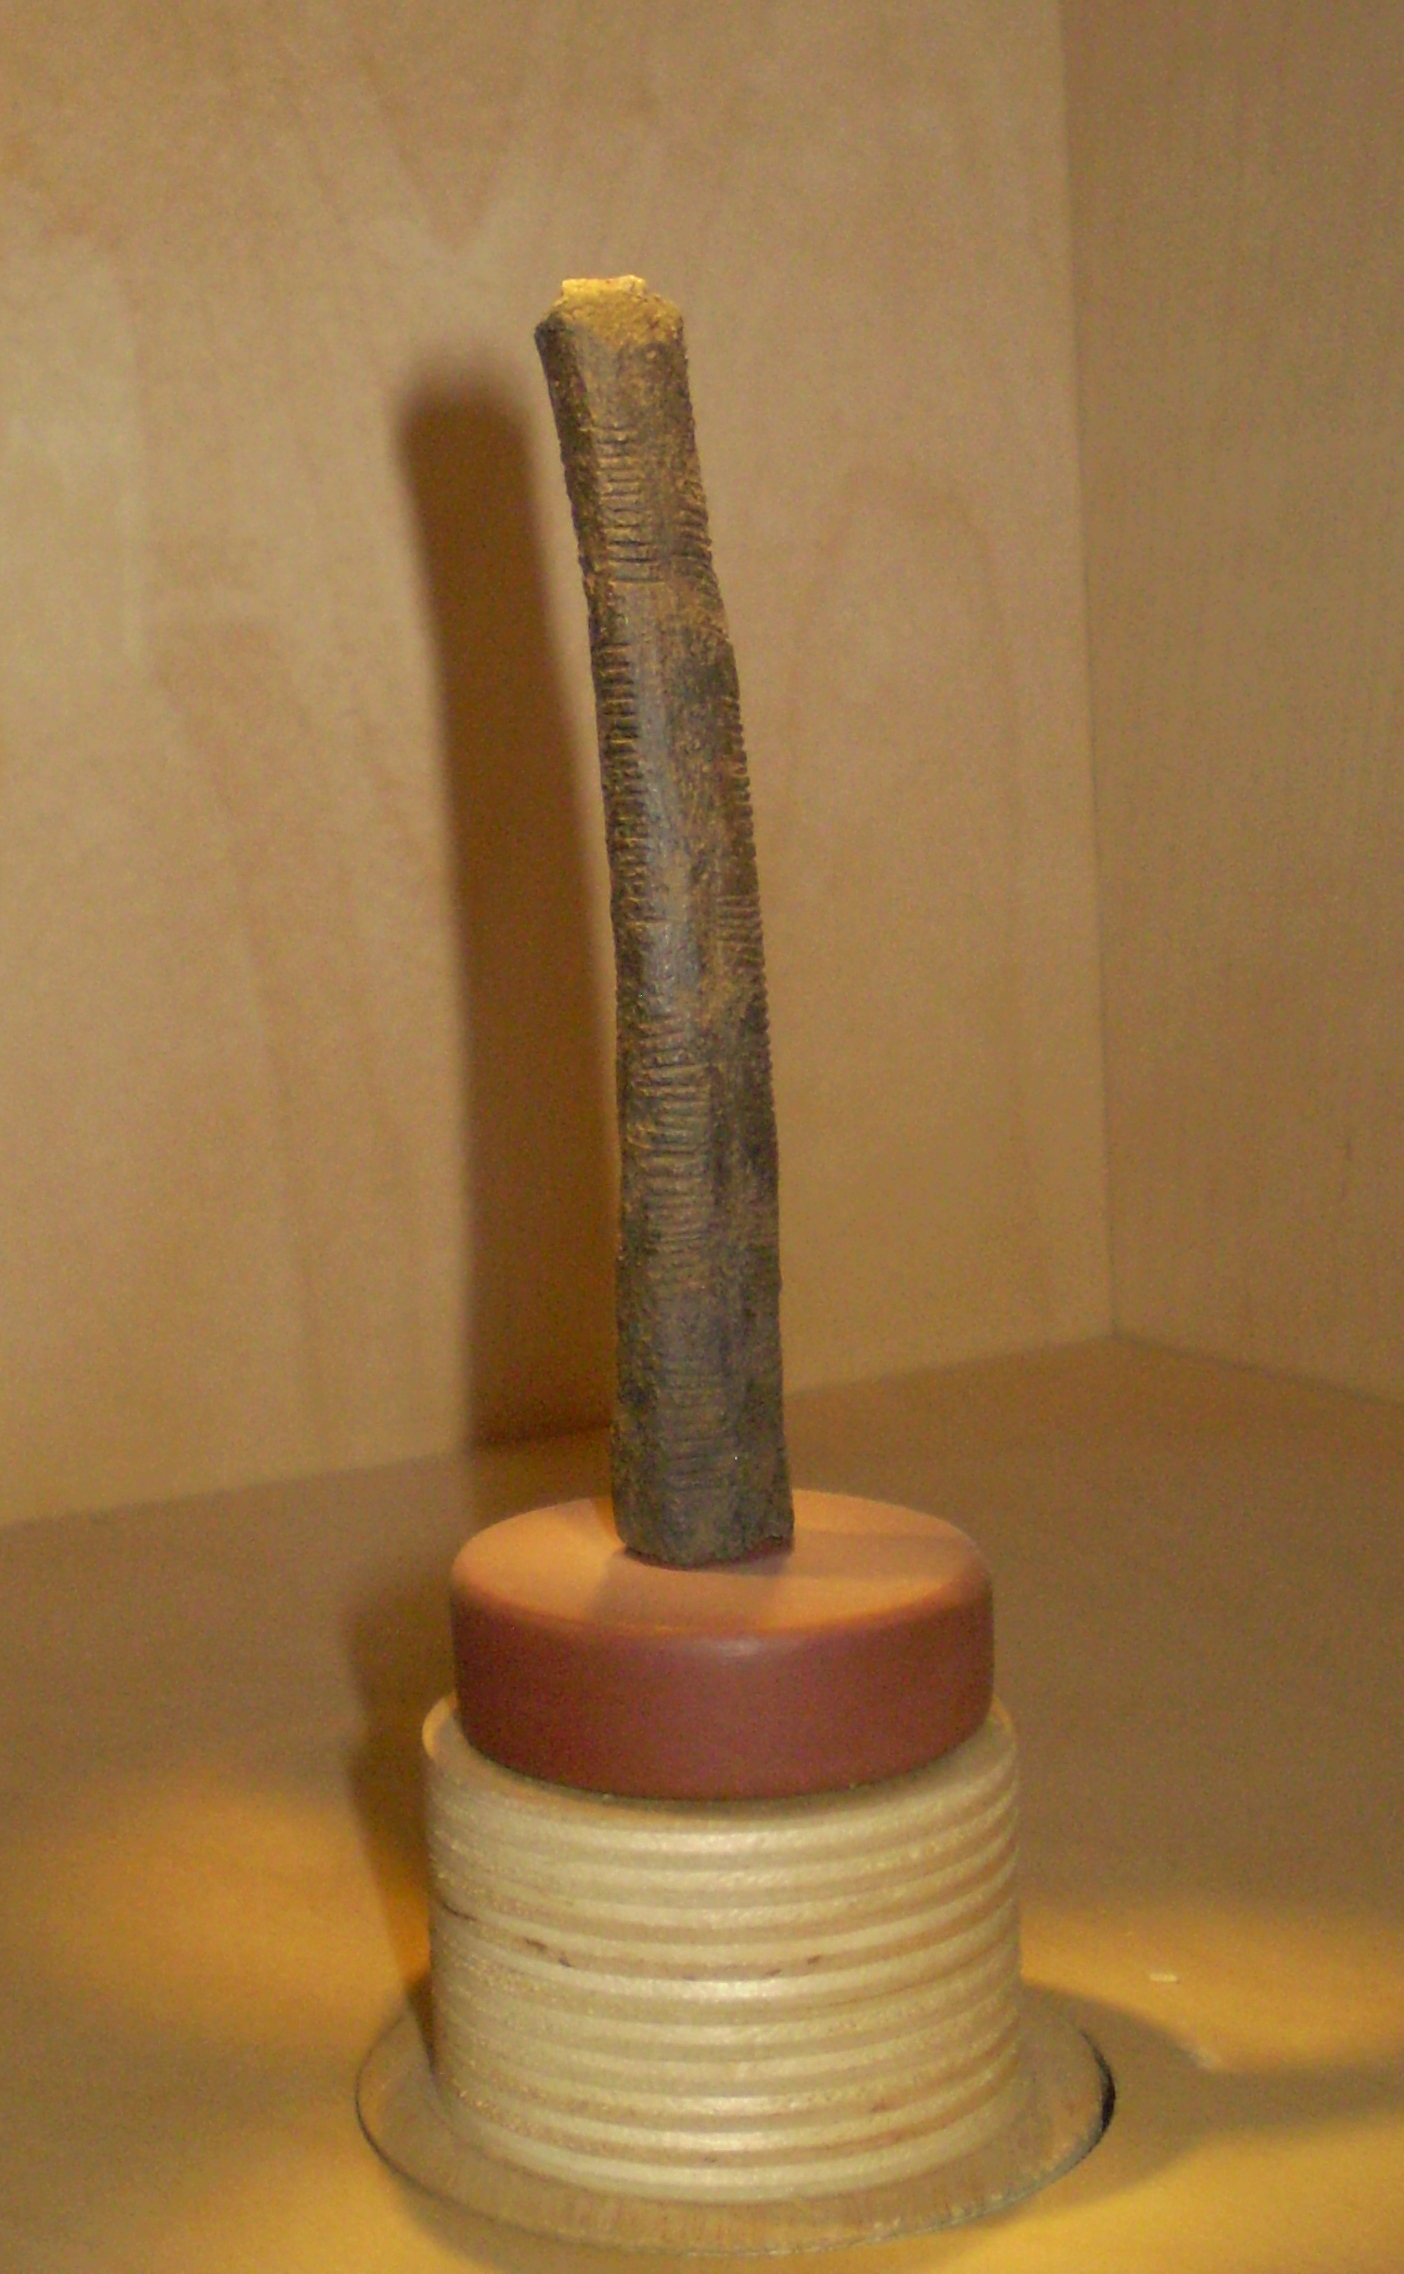
\includegraphics[width=0.22\textwidth]{../images/Os-Ishango.jpeg}
    %\caption{Os d'Ishango}
\end{wrapfigure}

Les os d'Ishango, également appelés bâtons d'Ishango, sont considérés comme le plus ancien outil de calcul jamais mis au jour. Ils ont été découverts au sein de vestiges archéologiques découverts dans l'ancien Congo belge. Le site est daté de plus de 20 000 ans. Selon certains auteurs, il pourrait s'agir de la plus ancienne attestation de la pratique de l'arithmétique dans l'histoire de l'humanité. Ils ont été considérés, dans un premier temps, comme des bâtons de comptage. 


\newpage

\textsc{ Jetons d'argile mésopotamiens} (~8000-3000 av. J.-C.) : 

\vspace{.2cm}

\begin{wrapfigure}[7]{l}{0.25\textwidth} % 8 = lignes occupées, l = à gauche
    \vspace{-0.6cm} % remonte l’image pour l’aligner avec la 1ère ligne du texte
    \includegraphics[width=0.25\textwidth]{../images/collier7800.jpg}
    %\caption{}
\end{wrapfigure}

Ces petits objets en forme de cônes, sphères ou disques servaient à compter les biens (bétail, céréales) avant l'invention de l'écriture. Les jetons d'argile mésopotamiens ont joué un rôle important dans le développement des systèmes de comptabilité et de commerce dès 8000 avant J.-C. Ces objets, dont la forme variait en fonction de l'objet qu'ils représentaient, étaient utilisés pour désigner et quantifier des marchandises.

\newpage


\textsc{ Tablettes cunéiformes babyloniennes} (~3000 av. J.-C.) : 

\vspace{.2cm}

\begin{wrapfigure}[5]{l}{0.55\textwidth} % 8 = lignes occupées, l = à gauche
    \vspace{-0.75cm} % remonte l’image pour l’aligner avec la 1ère ligne du texte
    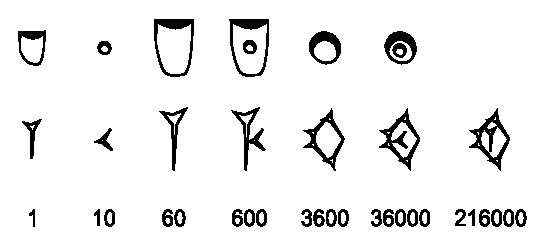
\includegraphics[width=0.55\textwidth]{../images/Proto-cuneiform-sexagesimal.pdf}
    %\caption{}
\end{wrapfigure}

Les premières traces écrites de calculs arithmétiques, avec un système sexagésimal (base 60) encore utilisé aujourd'hui pour mesurer le temps (1 heure = 60 minutes, 1 minute = 60 secondes, \dots ) et les angles (60 minutes = 1 degré).

\newpage

\textsc{ Papyrus de Rhind} (~2000 av. J.-C.):

\vspace{.2cm}

\begin{wrapfigure}[7]{l}{0.5\textwidth} % 8 = lignes occupées, l = à gauche
    \vspace{-0.75cm} % remonte l’image pour l’aligner avec la 1ère ligne du texte
    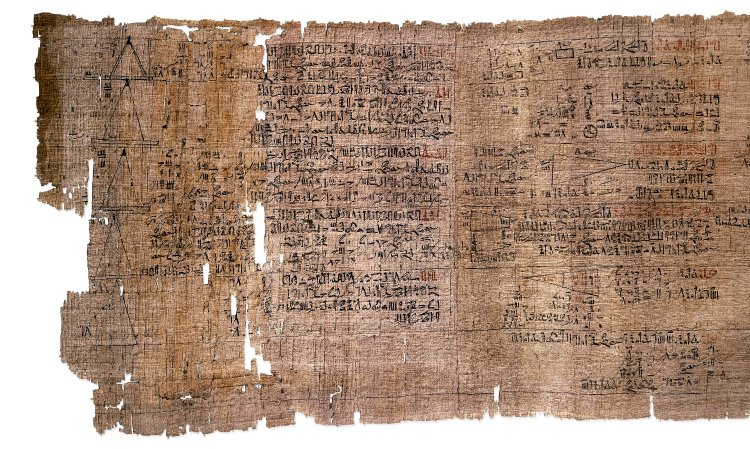
\includegraphics[width=0.5\textwidth]{../images/Rhind-Papyrus.jpg}
    %\caption{}
\end{wrapfigure}

Le papyrus Rhind, copié par Ahmès (Deuxième Période intermédiaire), synthétise les maths égyptiennes. Acheté par Rhind en 1858 à Louxor, il est au British Museum depuis 1865. Ce rouleau de 5 m (87 problèmes) couvre arithmétique, algèbre et géométrie, inspiré du Moyen Empire (2000 av. J.-C.). Son écriture hiératique en fait un document unique.


\newpage 


\subsection{Premières techniques de calcul}

\textsc{ L'abaque :} 

\vspace{.35cm}

\begin{wrapfigure}[7]{l}{0.55\textwidth} % 8 = lignes occupées, l = à gauche
    \vspace{-0.75cm} % remonte l’image pour l’aligner avec la 1ère ligne du texte
    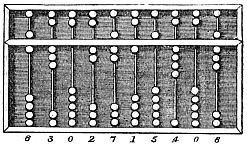
\includegraphics[width=0.55\textwidth]{../images/Abacus.png}
    %\caption{}
\end{wrapfigure}

Apparu vers 2700-2300 av. J.-C. en Mésopotamie, puis perfectionné par les Grecs et les Romains. Il permettait d'effectuer les quatre opérations fondamentales en déplaçant des jetons sur des lignes ou dans des colonnes.


\newpage

\textsc{ Le système décimal positionnel :} 

\vspace{.35cm}

\begin{wrapfigure}[12]{l}{0.6\textwidth} % 8 = lignes occupées, l = à gauche
    \vspace{-0.75cm} % remonte l’image pour l’aligner avec la 1ère ligne du texte
    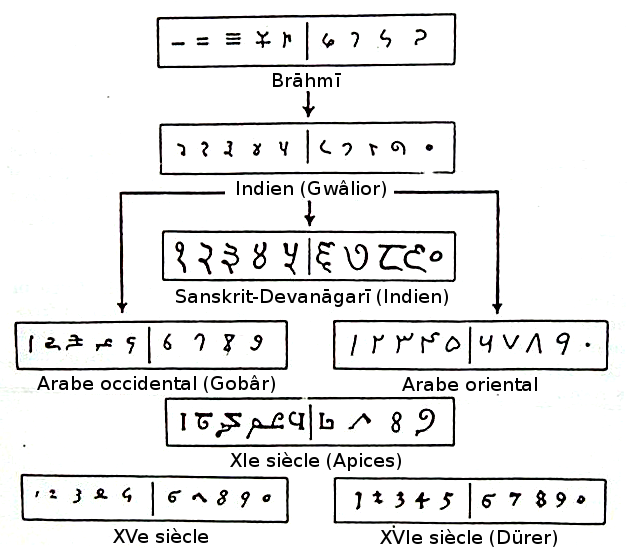
\includegraphics[width=0.6\textwidth]{../images/Numeration.png}
    %\caption{}
\end{wrapfigure}

Le système de numération indo-arabe est un système de numération de base dix employant une notation positionnelle et dix chiffres, allant de zéro à neuf, dont le tracé est indépendant de la valeur représentée. Dans ce système, la représentation d'un nombre correspond à son développement décimal. Le système doit son nom au fait qu'il est apparu en Inde et qu'il est parvenu en Europe par l'intermédiaire de mathématiciens et comptables de langue arabe. La variante graphique la plus répandue sont les chiffres utilisés en Europe, communément appelés chiffres arabes. Ce système tend aujourd’hui à s’imposer dans le monde.

\newpage

\textsc{ Les bâtons de Napier (1617) :} 

\vspace{.35cm}

\begin{wrapfigure}[8]{l}{0.45\textwidth} % 8 = lignes occupées, l = à gauche
    \vspace{-0.75cm} % remonte l’image pour l’aligner avec la 1ère ligne du texte
    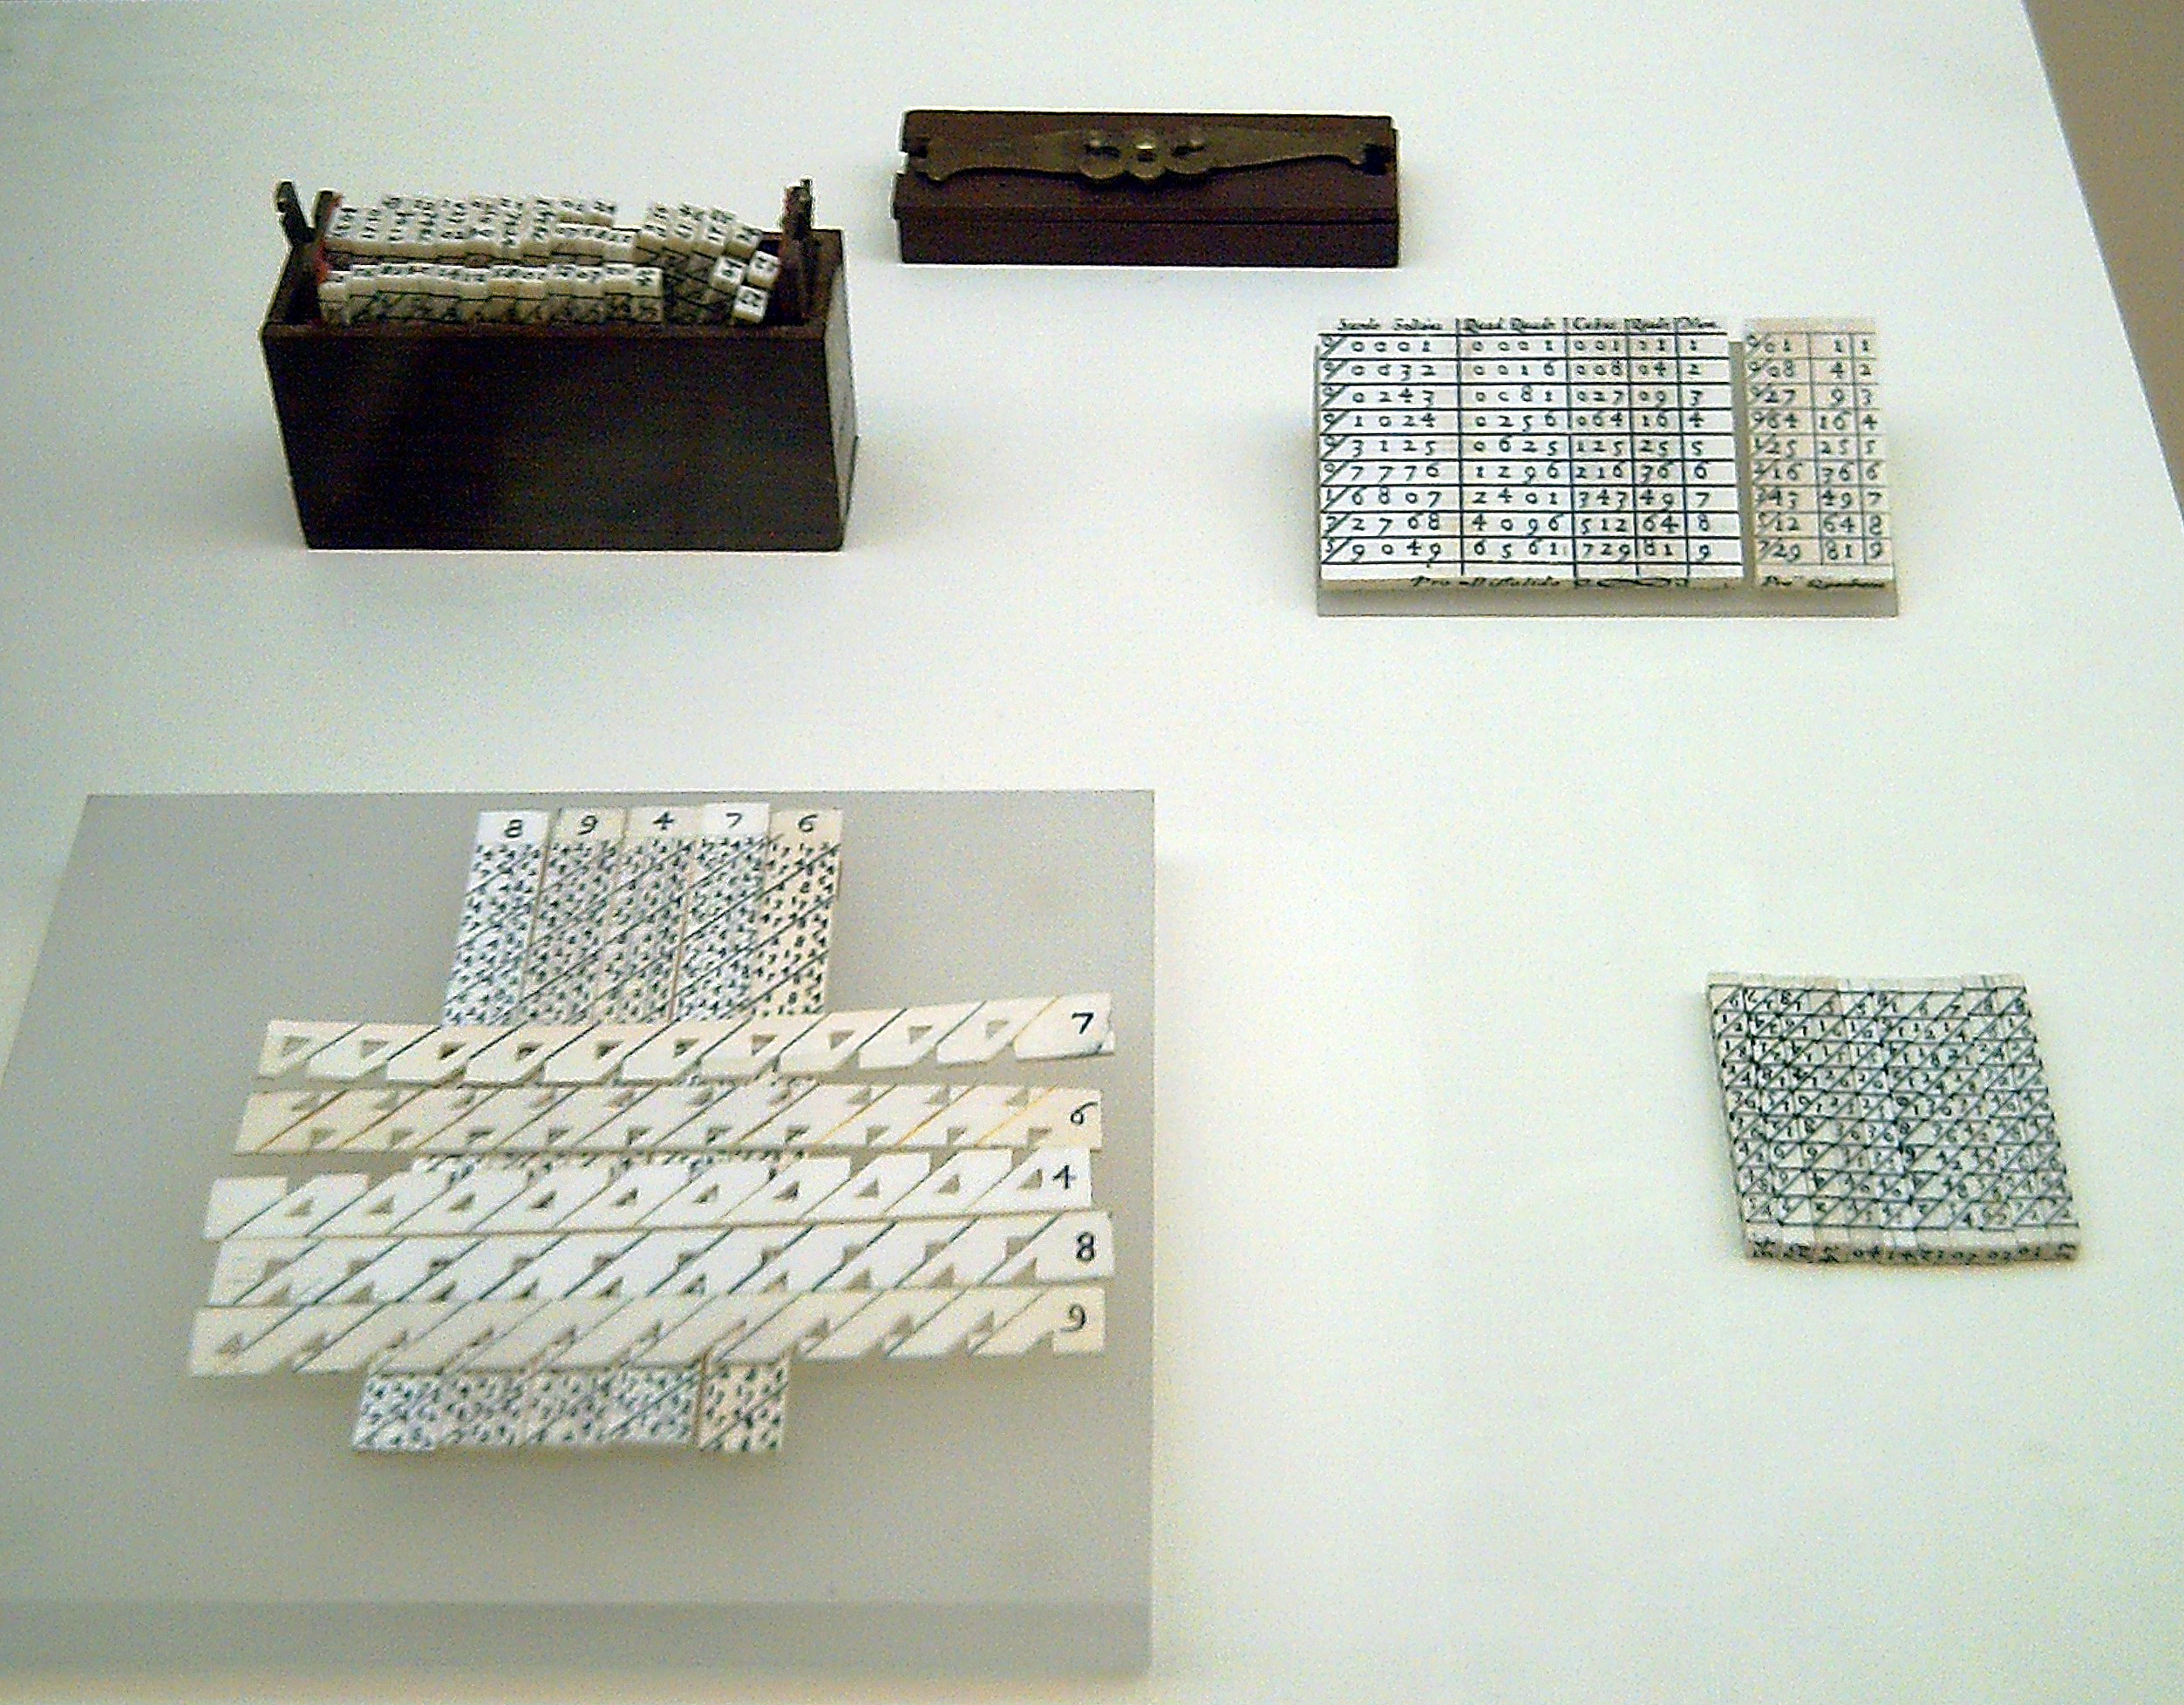
\includegraphics[width=0.45\textwidth]{../images/batons-napier.jpg}
    %\caption{}
\end{wrapfigure}

Le bâton de Napier, ou réglette de Neper est un abaque facilitant le calcul des produits, quotients, puissances et racines, inventé par le mathématicien écossais John Napier (en français Neper) en 1617.

L'abaque est constitué d'un plateau à rebord sur lequel peuvent être placées des réglettes gravées. Le bord gauche du plateau est gravé lui aussi, divisé en neuf cases numérotées de 1 à 9. Les dix types de réglettes, qui ont donné leur nom à l'ensemble du dispositif, étaient originellement en os, d'où le nom anglais de \textit{Napier's bones}. Elles sont divisées en neuf cases. La case supérieure porte un nombre de 0 à 9. Les huit autres cases sont divisées en deux par un trait diagonal.

\newpage

\textsc{ La pascaline (1642) :} 

\vspace{.35cm}

\begin{wrapfigure}[5]{l}{0.4\textwidth} % 8 = lignes occupées, l = à gauche
    \vspace{-0.75cm} % remonte l’image pour l’aligner avec la 1ère ligne du texte
    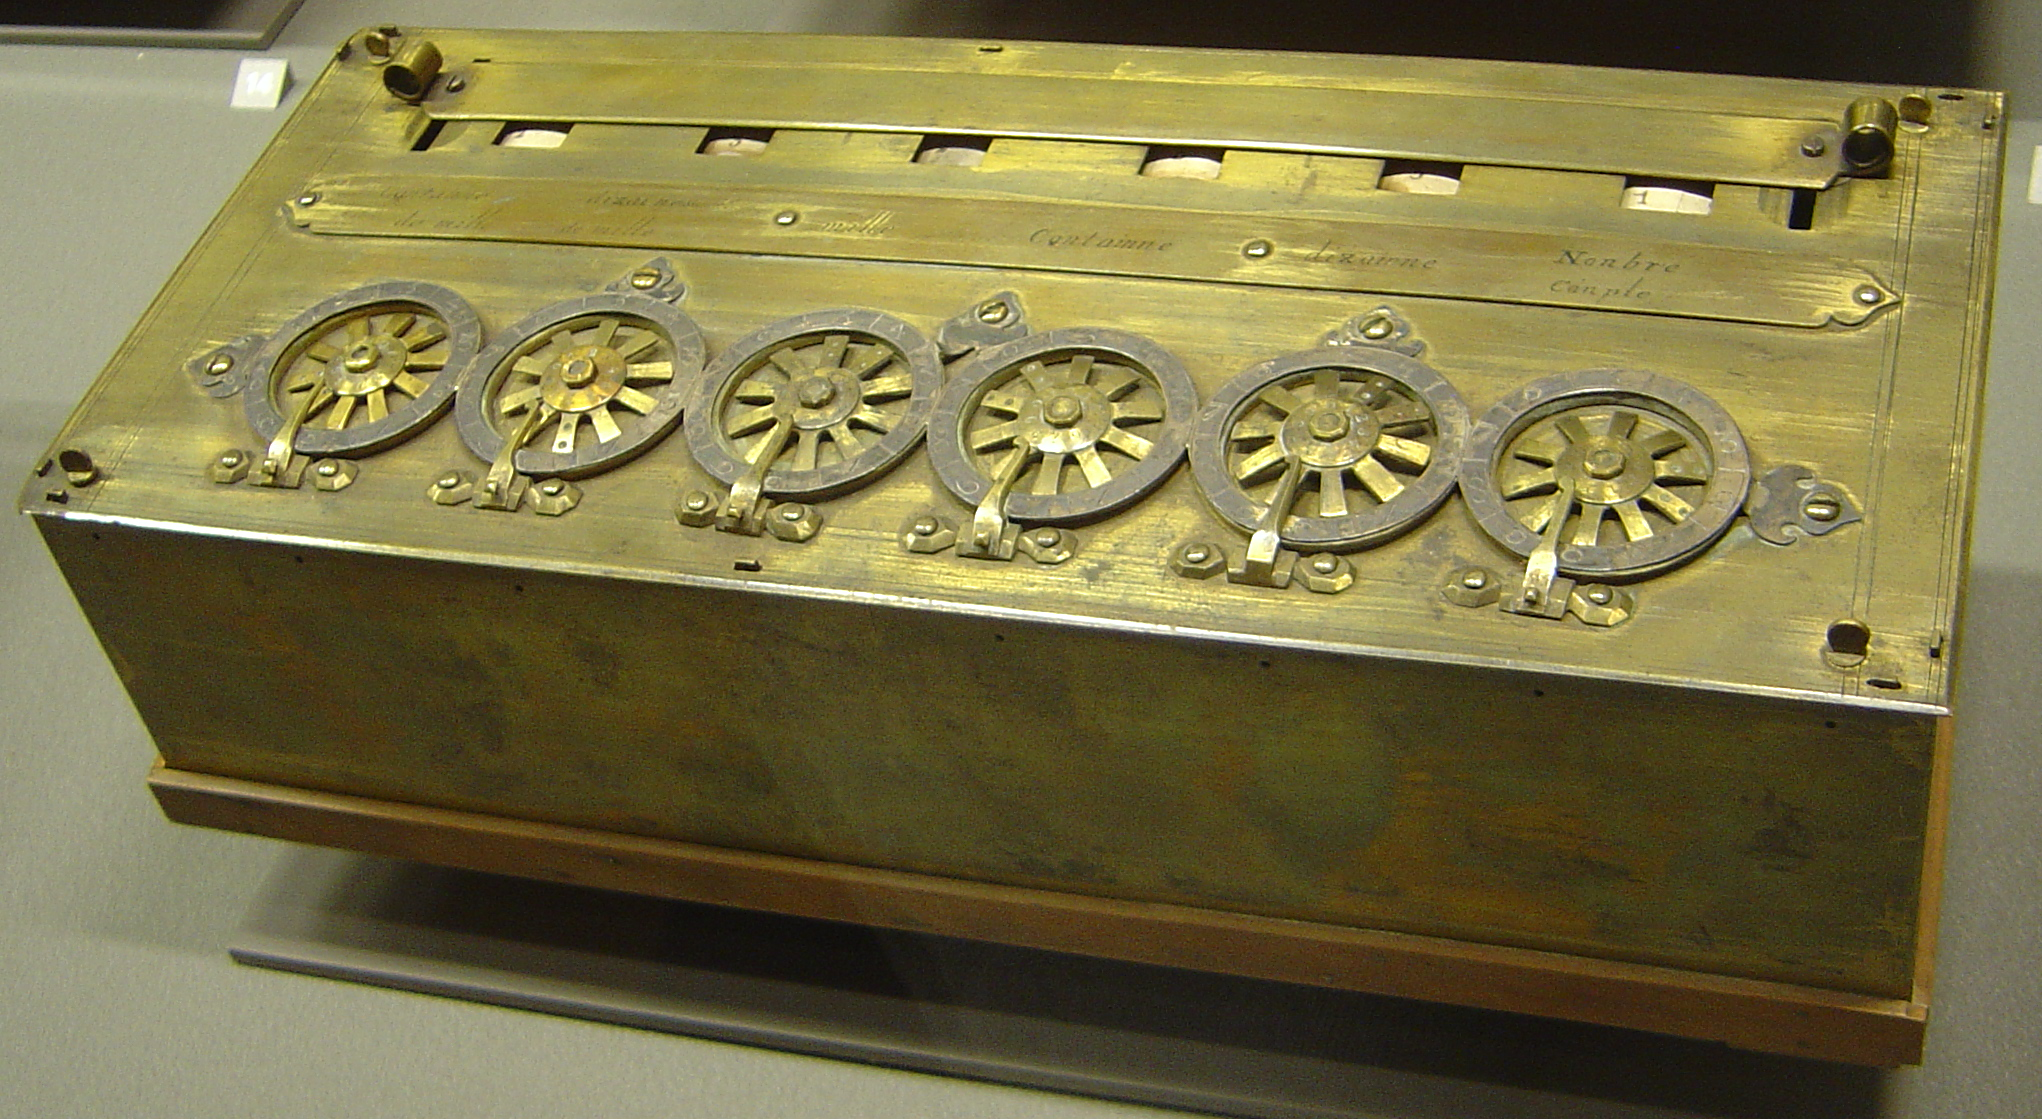
\includegraphics[width=0.4\textwidth]{../images/pascaline.jpg}
    %\caption{}
\end{wrapfigure}


La pascaline, initialement dénommée machine d’arithmétique puis roue pascaline, est une calculatrice mécanique inventée par Blaise Pascal et considérée comme la première machine à calculer. 


\newpage

\subsection{Les premières traces de géométrie}

Si les Grecs sont souvent vus comme les fondateurs de la géométrie en tant que science, de nombreuses connaissances en géométrie ont émergé bien avant eux, notamment vers 3000 av. J.-C., en Égypte ancienne, en Mésopotamie et dans l'Inde antique, pour répondre à des besoins pratiques en agriculture, astronomie, architecture et topographie.

\vspace{.5cm}



\textsc{Manuscript de Bakhshali} (Civilisation de la vallée de l'Indus) : 

\vspace{.2cm}

\begin{wrapfigure}[6]{l}{0.5\textwidth} % 6 = lignes occupées, l = à gauche
    \vspace{-0.65cm} % remonte l’image pour l’aligner avec la 1ère ligne du texte
    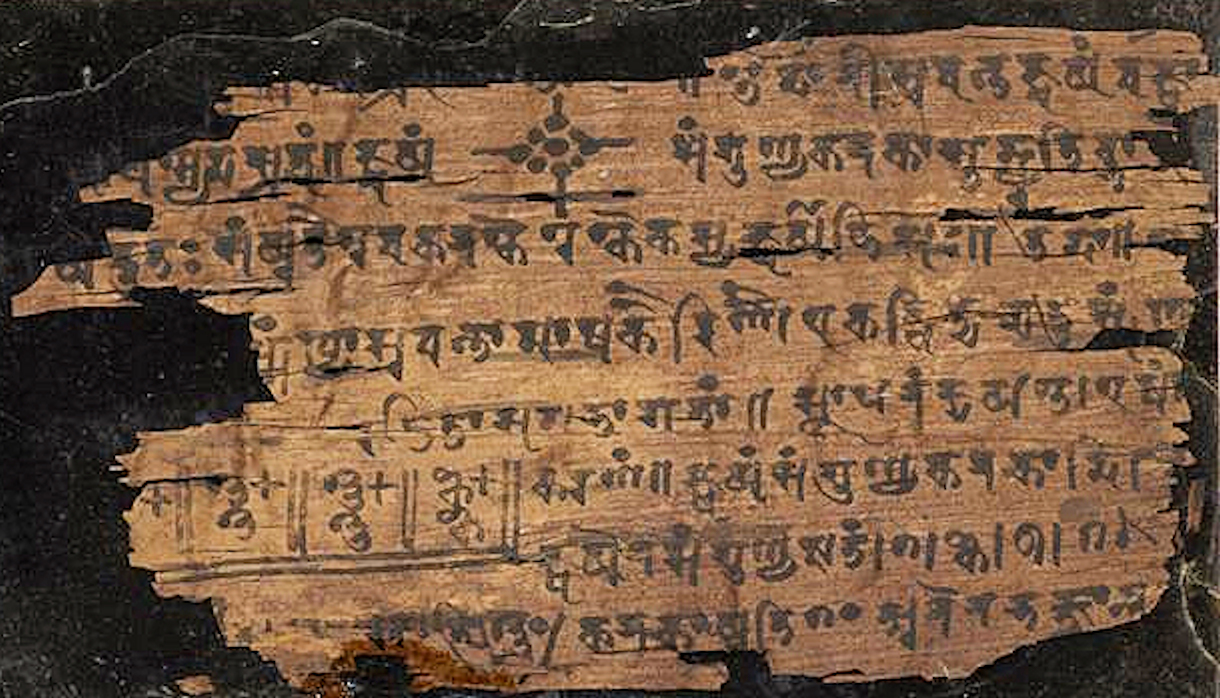
\includegraphics[width=0.5\textwidth]{../images/Bakhshali_manuscript.jpg}
    %\caption{Os d'Ishango}
\end{wrapfigure}

La civilisation de la vallée de l'Indus, attestée dès environ -3300, livre les premiers indices d'une activité mathématique en Inde. Les découvertes effectuées à Harappa, Mohenjo-daro et dans leur environnement révèlent un système de poids et mesures précis et décimal datant d’environ 2600 avant J.-C., une technologie de fabrication de briques basée sur des proportions rigoureuses, ainsi qu’une attention aux formes géométriques.


\newpage


\textsc{Tablette babylonienne YBC 7289} (Babylone) : 

\vspace{.2cm}

\begin{wrapfigure}[10]{l}{0.5\textwidth} % 10 = lignes occupées, l = à gauche
    \vspace{-0.65cm} % remonte l’image pour l’aligner avec la 1ère ligne du texte
    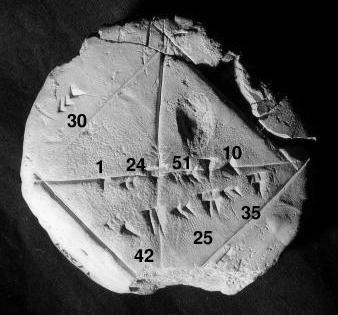
\includegraphics[width=0.5\textwidth]{../images/Ybc7289.jpg}
    %\caption{Os d'Ishango}
\end{wrapfigure}

La tablette YBC 7289 a probablement été rédigée par un scribe babylonien de la première dynastie, entre 1900 et 1600 avant J.-C. Elle aurait été écrite dans le sud de l’actuel Irak, vraisemblablement par un apprenti utilisant des valeurs tirées d’une liste connue. De forme ronde et compacte (8 à 12 cm environ), elle était facile à tenir en main. 

La suite de nombres est à interpréter de la façon suivante : 
\begin{align*}
1 + \dfrac{24}{60} + \dfrac{51}{60^2} + \dfrac{10}{60^3} &\simeq \sqrt{2}\\
42 + \dfrac{25}{60} + \dfrac{35}{60^2} &\simeq 30\sqrt{2}
\end{align*}

\newpage


\textsc{Papyrus de Moscou} (Civilisation Egyptienne) : 

\vspace{.2cm}

\begin{wrapfigure}[7]{l}{0.65\textwidth} % 7 = lignes occupées, l = à gauche
    \vspace{-0.65cm} % remonte l’image pour l’aligner avec la 1ère ligne du texte
    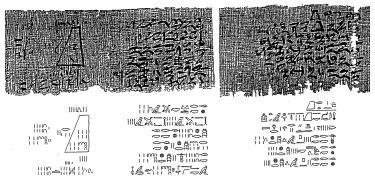
\includegraphics[width=0.65\textwidth]{../images/papyrus-moscou.jpg}
    %\caption{Os d'Ishango}
\end{wrapfigure}

Écrit vers 1850 av. J.-C., pendant la XIe dynastie, le papyrus de Moscou est un exemple ancien d’étude mathématique utilisant le système unaire. Long d’environ 5,40 mètres et large de 4 à 7 cm, il contient 25 problèmes résolus, dont certains portent sur la surface d’une demi-sphère et le volume d’une pyramide tronquée.


\newpage


\textsc{Les Neuf Chapitres sur l'art mathématique} (Civilisation Chinoise après les Grecs) : 

\vspace{.2cm}

\begin{wrapfigure}[10]{l}{0.35\textwidth} % 10 = lignes occupées, l = à gauche
    \vspace{-0.65cm} % remonte l’image pour l’aligner avec la 1ère ligne du texte
    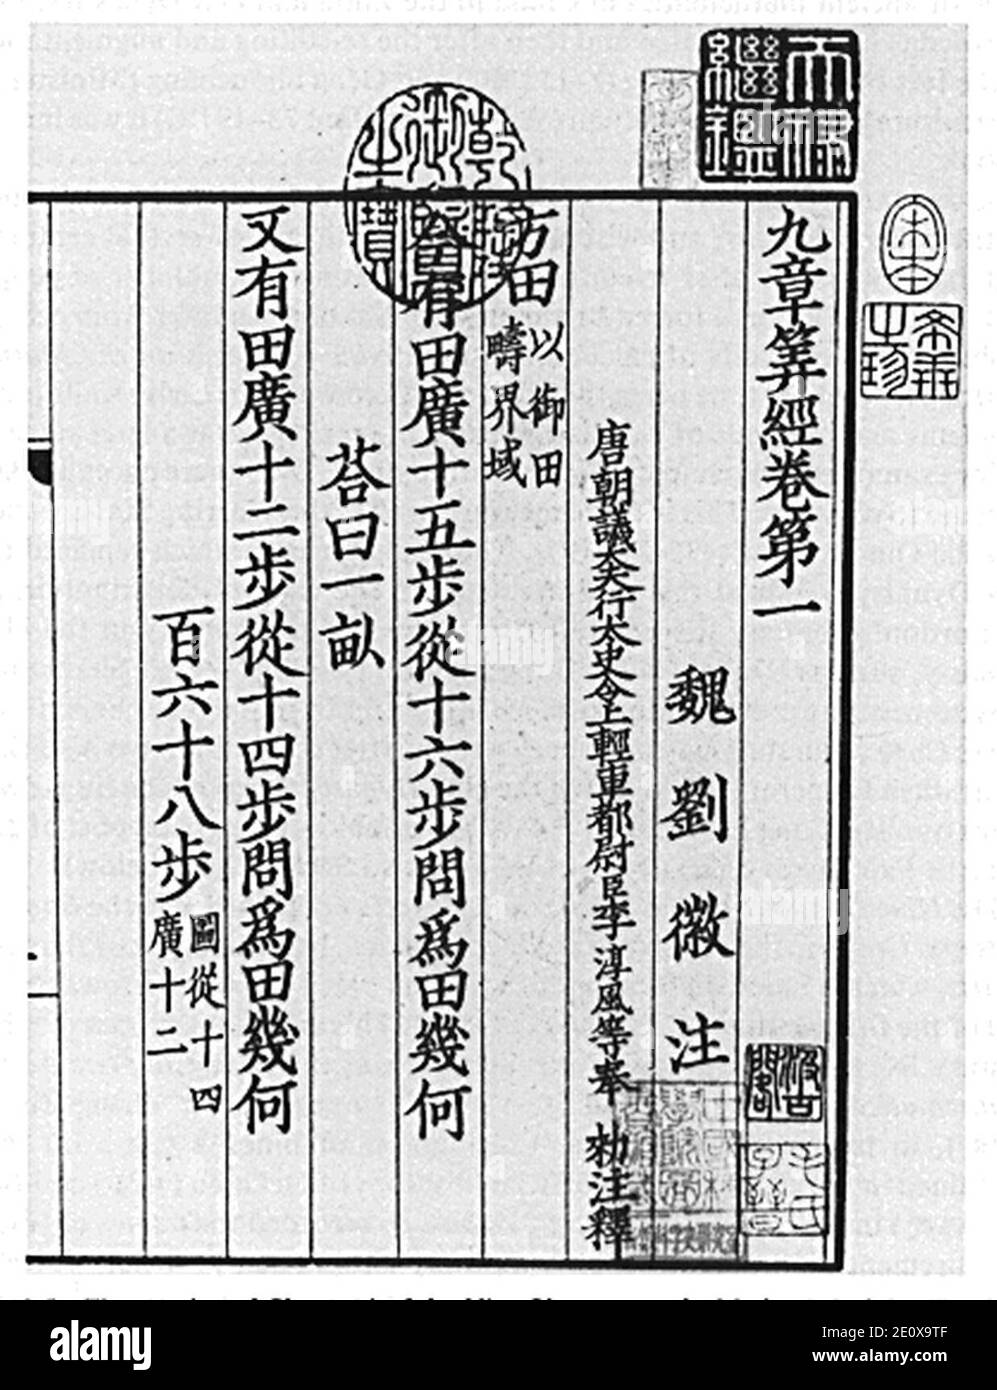
\includegraphics[width=0.35\textwidth]{../images/9chap.jpg}
    %\caption{Os d'Ishango}
\end{wrapfigure}

Les Neuf Chapitres sur l’art mathématique forment un ouvrage chinois anonyme compilé entre le IIe et le Ier siècle av. J.-C., au début de la dynastie Han. Reprenant des textes antérieurs, il propose une approche méthodique des mathématiques à travers des techniques générales de résolution de problèmes. Connu grâce aux copies des scribes puis à l’imprimerie, il fut commenté notamment par Liu Hui en 263.


\newpage



\hypertarget{chap:level1}{}
\chapter{Niveau primaire}\label{chap:level1}

\section{Calculs niveau primaire}
\addcontentsline{toc}{chapter}{Calculs niveau primaire}

Pour les séries de calculs ci-dessous, essayez de les faire de tête. Si vous n'y arrivez pas alors posez-les à la main. Et si vous n'y arrivez toujours pas vérifiez avec une calculatrice. 

\newpage

\subsection{Exercice 1 (primaire) : Additions simples}


\label{calc:niveau1}

\begin{enumerate}[label=C\arabic*)]
    \item 5 + 3 = \_\_\_
    \item 9 + 2 = \_\_\_
    \item 7 + 6 = \_\_\_
    \item 4 + 8 = \_\_\_
    \item 3 + 9 = \_\_\_
    \item 1 + 7 = \_\_\_
    \item 2 + 3 = \_\_\_
    \item 3 + 4 = \_\_\_
    \item 4 + 5 = \_\_\_
    \item 5 + 6 = \_\_\_
    \item 1 + 9 = \_\_\_
    \item 9 + 2 = \_\_\_
    \item 2 + 8 = \_\_\_
    \item 8 + 3 = \_\_\_
    \item 3 + 9 = \_\_\_
    \item 9 + 7 = \_\_\_
    \item 7 + 8 = \_\_\_
    \item 8 + 5 = \_\_\_
    \item 5 + 9 = \_\_\_
    \item 5 + 7 = \_\_\_
\end{enumerate}

\hyperref[sol:niveau1]{Voir solutions des additions page \pageref{sol:niveau1}}.

\newpage


\subsection{Exercice 2 (primaire) : Soustractions}


\label{calc:niveau2}

\begin{enumerate}[label=C\arabic*)]
    \item 15 - 7 = \_\_\_
    \item 18 - 9 = \_\_\_
    \item 12 - 4 = \_\_\_
    \item 20 - 11 = \_\_\_
    \item 17 - 8 = \_\_\_
    \item 30 - 15 = \_\_\_
    \item 49 - 26 = \_\_\_
    \item 58 - 37 = \_\_\_
    \item 67 - 48 = \_\_\_
    \item 76 - 59 = \_\_\_
    \item 51 - 17 = \_\_\_
    \item 81 - 29 = \_\_\_
    \item 21 - 14 = \_\_\_
    \item 30 - 11 = \_\_\_
    \item 47 - 18 = \_\_\_
    \item 50 - 15 = \_\_\_
    \item 94 - 62 = \_\_\_
    \item 85 - 73 = \_\_\_
    \item 76 - 48 = \_\_\_
    \item 67 - 59 = \_\_\_
\end{enumerate}

\hyperref[sol:niveau2]{Voir solutions des soustractions page \pageref{sol:niveau2}}.

\newpage


\subsection{Exercice 3 (primaire) : Multiplications à 1 chiffre}


\label{calc:niveau3}

\begin{enumerate}[label=C\arabic*)]
    \item \(3\times 4 = \_\_\_\)
    \item \(6\times 7 = \_\_\_\)
    \item \(8\times 5 = \_\_\_\)
    \item \(9\times 3 = \_\_\_\)
    \item \(2\times 6 = \_\_\_\)
    \item \(6\times 5 = \_\_\_\)
    \item \(7\times 6 = \_\_\_\)
    \item \(8\times 9 = \_\_\_\)
    \item \(2\times 8 = \_\_\_\)
    \item \(7\times 3 = \_\_\_\)
    \item \(2\times 2 = \_\_\_\)
    \item \(3\times 3 = \_\_\_\)
    \item \(4\times 4 = \_\_\_\)
    \item \(5\times 5 = \_\_\_\)
    \item \(6\times 6 = \_\_\_\)
    \item \(7\times 7 = \_\_\_\)
    \item \(8\times 8 = \_\_\_\)
    \item \(9\times 9 = \_\_\_\)
    \item \(5\times 7 = \_\_\_\)
    \item \(7\times 8 = \_\_\_\)
\end{enumerate}

\hyperref[sol:niveau3]{Voir solutions des multiplications à 1 chiffre page \pageref{sol:niveau3}}.

\newpage


\subsection{Exercice 4 (primaire) : Multiplications à 2 chiffres par 11}


\label{calc:niveau4}

\begin{enumerate}[label=C\arabic*)]
    \item \(11\times 12 = \_\_\_\)
    \item \(11\times 23 = \_\_\_\)
    \item \(11\times 34 = \_\_\_\)
    \item \(11\times 45 = \_\_\_\)
    \item \(11\times 56 = \_\_\_\)
    \item \(11\times 67 = \_\_\_\)
    \item \(11\times 78 = \_\_\_\)
    \item \(11\times 89 = \_\_\_\)
    \item \(11\times 13 = \_\_\_\)
    \item \(11\times 24 = \_\_\_\)
    \item \(99\times 11 = \_\_\_\)
    \item \(89\times 11 = \_\_\_\)
    \item \(78\times 11 = \_\_\_\)
    \item \(65\times 11 = \_\_\_\)
    \item \(54\times 11 = \_\_\_\)
    \item \(46\times 11 = \_\_\_\)
    \item \(37\times 11 = \_\_\_\)
    \item \(29\times 11 = \_\_\_\)
    \item \(19\times 11 = \_\_\_\)
    \item \(91\times 11 = \_\_\_\)
\end{enumerate}

\hyperref[sol:niveau4]{Voir solutions des multiplications à 2 chiffres par 11 page \pageref{sol:niveau4}}.

\newpage


\subsection{Exercice 5 (primaire) : Divisions à 1 chiffre}


\label{calc:niveau5}

\begin{enumerate}[label=C\arabic*)]
    \item \(9 \div 3 =  \_\_\_\)
    \item \(8 \div 2 = \_\_\_\)
    \item \(6 \div 3 = \_\_\_\)
    \item \(4 \div 2 = \_\_\_\)
    \item \(6 \div 2 = \_\_\_\)
    \item \(8 \div 4 = \_\_\_\)
    \item \(9 \div 9 = \_\_\_\)
    \item \(8 \div 1 = \_\_\_\)
    \item \(5 \div 5 = \_\_\_\)
    \item \(7 \div 7 = \_\_\_\)
    \item \(18 \div 9 =  \_\_\_\)
    \item \(18 \div 6 = \_\_\_\)
    \item \(18 \div 3 = \_\_\_\)
    \item \(16 \div 2 = \_\_\_\)
    \item \(16 \div 4 = \_\_\_\)
    \item \(16 \div 8 = \_\_\_\)
    \item \(12 \div 2 = \_\_\_\)
    \item \(12 \div 3 = \_\_\_\)
    \item \(12 \div 4 = \_\_\_\)
    \item \(12 \div 6 = \_\_\_\)
\end{enumerate}

\hyperref[sol:niveau5]{Voir solutions des divisions à 1 chiffre page \pageref{sol:niveau5}}.

\newpage


\subsection{Exercice 6 (primaire) : Divisions à 2 chiffres}


\label{calc:niveau6}

\begin{enumerate}[label=C\arabic*)]
    \item \(99 \div 11 =  \_\_\_\)
    \item \(84 \div 12 = \_\_\_\)
    \item \(72 \div 18 = \_\_\_\)
    \item \(64 \div 16 = \_\_\_\)
    \item \(56 \div 28 = \_\_\_\)
    \item \(42 \div 14 = \_\_\_\)
    \item \(36 \div 12 = \_\_\_\)
    \item \(24 \div 12 = \_\_\_\)
    \item \(39 \div 13 = \_\_\_\)
    \item \(45 \div 15 = \_\_\_\)
    \item \(54 \div 27 =  \_\_\_\)
    \item \(63 \div 21 = \_\_\_\)
    \item \(74 \div 37 = \_\_\_\)
    \item \(82 \div 41 = \_\_\_\)
    \item \(98 \div 49 = \_\_\_\)
    \item \(80 \div 20 = \_\_\_\)
    \item \(92 \div 23 = \_\_\_\)
    \item \(93 \div 31 = \_\_\_\)
    \item \(69 \div 23 = \_\_\_\)
    \item \(55 \div 11 = \_\_\_\)
\end{enumerate}


\hyperref[sol:niveau6]{Voir solutions des divisions à 2 chiffres page \pageref{sol:niveau6}}.

\newpage



\hypertarget{chap:level2}{}
\chapter{Niveau secondaire : collège}\label{chap:level2}

\section{Calculs niveau collège}
\addcontentsline{toc}{chapter}{Calculs niveau collège}

Dans cette partie, on commence dans la continuité de la partie précédente avec des calculs purs et durs mais déjà vous devriez pouvoir trouver des astuces de calculs. Cela signifie que le raisonnement commence à jouer un rôle utile. Ensuite, on passera au calcul littéral, puis sa liaison avec la géométrie. Et de la géométrie on en viendra aux probabilités. 

\newpage

\subsection{Exercice 7 (secondaire : collège) : carrés}


\label{calc:niveau7}

\begin{enumerate}[label=C\arabic*)]
    \item \(11^2 = 11 \times 11 =  \_\_\_\)
    \item \(12^2 = 12 \times 12 = \_\_\_\)
    \item \(13^2 = 13 \times 13 = \_\_\_\)
    \item \(14^2 = 14 \times 14 = \_\_\_\)
    \item \(15^2 = 15 \times 15 = \_\_\_\)
    \item \(16^2 = 16 \times 16 = \_\_\_\)
    \item \(17^2 = 17 \times 17 = \_\_\_\)
    \item \(18^2 = 18 \times 18 = \_\_\_\)
    \item \(19^2 = 19 \times 19 = \_\_\_\)
    \item \(20^2 = 20 \times 20 = \_\_\_\)
    \item \(25^2 = 25 \times 25 =  \_\_\_\)
    \item \(35^2 = 35 \times 35 = \_\_\_\)
    \item \(45^2 = 45 \times 45 = \_\_\_\)
    \item \(55^2 = 55 \times 55 = \_\_\_\)
    \item \(65^2 = 65 \times 65 = \_\_\_\)
    \item \(75^2 = 75 \times 75 = \_\_\_\)
    \item \(85^2 = 85 \times 85 = \_\_\_\)
    \item \(95^2 = 95 \times 95 = \_\_\_\)
    \item \(111^2 = 111 \times 111 = \_\_\_\)
    \item \(1111^2 = 1111 \times 1111 = \_\_\_\)
\end{enumerate}




\hyperref[sol:niveau7]{Voir solutions des calculs de carrés page \pageref{sol:niveau7}}.

\newpage

\subsection{Exercice 8 (secondaire : collège) : carrés avec des 1 et une calculatrice}


\label{calc:niveau8}

\begin{enumerate}[label=C\arabic*)]
    \item \(1^2 = 1 \times 1 =  \_\_\_\)
    \item \(11^2 = 11 \times 11 = \_\_\_\)
    \item \(111^2 = 111 \times 111 = \_\_\_\)
    \item \(1111^2 = 1111 \times 1111 = \_\_\_\)
    \item \(11111^2 = 11111 \times 11111 = \_\_\_\)
    \item \(111111^2 = 111111 \times 111111 = \_\_\_\)
    \item \(1111111^2 = 1111111 \times 1111111 = \_\_\_\)
    \item \(11111111^2 = 11111111 \times 11111111 = \_\_\_\)
    \item \(111111111^2 = 111111111 \times 111111111 = \_\_\_\)
    \item \(1111111111^2 = 1111111111 \times 1111111111 = \_\_\_\)
\end{enumerate}

\hyperref[sol:niveau8]{Voir solutions des calculs de carrés page \pageref{sol:niveau8}}.


\newpage 

\subsection{Exercice 9 (secondaire : collège) : Un programme de calcul particulier}

\label{calc:niveau9}

Considérons le programme de calcul suivant :

\begin{enumerate}[label=P\arabic*)]
	\item Choisir un nombre entier strictement supérieur à 1 (\(m > 1\) par exemple 2, 3, 4\dots ) 
	\item Choisir un autre nombre entier strictement positif \(n\) strictement inférieur à \(m\quad n < m\)
	\item Calculer le nombre \(a\) comme la différence du carré de \(m\) avec le carré de \(n\), concrètement \(a = m^2 - n^2\)
	\item Calculer le nombre \(b\) comme le double du produit de \(m\) et de \(n\), concrètement \(b = 2mn\)
	\item Calculer le nombre \(c\) comme la somme du carré de \(m\) avec le carré de \(n\), concrètement \(c = m^2 + n^2\)
	\item Calculer le carré de \(a\)
	\item Calculer le carré de \(b\)
	\item Calculer le carré de \(c\)
	\item Calculer la somme du carré de \(a\) et celui de \(b\)
	\item Comparer cette somme avec le carré de \(c\)
\end{enumerate}

\newpage

Appliquons le programme de calcul ci-dessus avec les nombres \(m = 2\) et \(n = 1\) : 

\begin{enumerate}[label=C\arabic*)]
    \item \(m^2 = 2 \times 2 =  \_\_\_\)
    \item \(n^2 = 1 \times 1 = \_\_\_\)
    \item \(a = m^2 - n^2 = \_\_\_\)
    \item \(b = 2 \times m \times n = \_\_\_\)
    \item \(c = m^2 + n^2 = \_\_\_\)
    \item \(a^2 =  \_\_\_\)
    \item \(b^2 =  \_\_\_\)
    \item \(c^2 =  \_\_\_\)
    \item Vérifiez que \( a^2 + b^2 = c^2 \)
    \item Est-ce valable pour n'importe quelles valeurs de \(m\) et \(n\) ?
\end{enumerate}


\hyperref[sol:niveau9]{Voir solutions des calculs du programme page \pageref{sol:niveau9}}.

\newpage 

\subsection{Exercice 10 (secondaire : collège) : Un programme de construction géométrique, Pythagore}

\label{geom:niveau10}

\begin{enumerate}[label=G\arabic*)]
	\item Dans un repère orthonormé placer le point \(A\) de coordonnées \((-1 ; -2)\) c'est-à-dire d'abscisse \(x_A = -1\) et d'ordonnée \(y_A = -2\)
	\item Placer le point \(B\) de coordonnées \((2 ; -2)\) c'est-à-dire d'abscisse \(x_B = 2\) et d'ordonnée \(y_B = -2\)
	\item Placer le point \(C\) de coordonnées \((2 ; 2)\) c'est-à-dire d'abscisse \(x_C = 2\) et d'ordonnée \(y_C = 2\)
	\item En utilisant le théorème de Pythagore vérifier que le carré ABC est rectangle en B.
\end{enumerate}

\hyperref[sol:niveau10]{Voir solution du programme de construction géométrique page \pageref{sol:niveau10}}.

\newpage


\subsection{Exercice 11 (secondaire : collège) : Un cible circulaire, probabilités}

\label{proba:niveau11}

Considérons la cible définie par les cercles concentriques sur le schéma ci-dessous : 
\definecolor{yellow}{rgb}{1,0.8,0.2}
\definecolor{orange}{rgb}{1,0.5,0}
\definecolor{navy}{rgb}{0,0,1}
\definecolor{lime}{rgb}{0,1,0}
\definecolor{red}{rgb}{1,0,0}
\definecolor{black}{rgb}{0,0}

\begin{figure}[H]
\centering
\caption{Cible de cercles concentriques}
\vspace{.25cm}
\begin{tikzpicture}[line cap=round,line join=round,>=triangle 45,x=1cm,y=1cm]
\begin{axis}[
x=1cm,y=1cm,
axis lines=middle,
ymajorgrids=true,
xmajorgrids=true,
xmin=-5.5,
xmax=5.5,
ymin=-5.5,
ymax=5.5,
xtick={-5, -4,...,5},
ytick={-5,-4,...,5},]
\clip(-5.5,-5.5) rectangle (6,5.5);
\draw [line width=2pt,color=red] (0,0) circle (1cm);
\draw [line width=2pt,color=lime] (0,0) circle (2cm);
\draw [line width=2pt,color=navy] (0,0) circle (3cm);
\draw [line width=2pt,color=orange] (0,0) circle (4cm);
\draw [line width=2pt,color=yellow] (0,0) circle (5cm);
\begin{scriptsize}
\draw [fill=black] (0,0) circle (2.5pt);
\draw[color=black] (0.14280352603970045,0.37709534368070763) node {$O$};
\draw [fill=red] (1,0) circle (2.5pt);
\draw[color=red] (1.25,0.38) node {$A$};
\draw[color=red] (1.05,1.05) node {$(\mathcal{C}_A)$};
\draw [fill=lime] (2,0) circle (2.5pt);
\draw[color=lime] (2.25,0.38) node {$B$};
\draw[color=lime] (1.75,1.75) node {$(\mathcal{C}_B)$};
\draw [fill=navy] (3,0) circle (2.5pt);
\draw[color=navy] (3.25,0.378) node {$C$};
\draw[color=navy] (2.5,2.5) node {$(\mathcal{C}_C)$};
\draw [fill=orange] (4,0) circle (2.5pt);
\draw[color=orange] (4.25,0.378) node {$D$};
\draw[color=orange] (3.15,3.15) node {$(\mathcal{C}_D)$};
\draw [fill=yellow] (5,0) circle (2.5pt);
\draw[color=yellow] (5.25,0.378) node {$E$};
\draw[color=yellow] (3.9,3.9) node {$(\mathcal{C}_E)$};
\end{scriptsize}
\end{axis}
\end{tikzpicture}
\label{fig:proba-target}
\end{figure}

\newpage

\definecolor{yellow}{rgb}{1,0.8,0.2}
\definecolor{orange}{rgb}{1,0.5,0}
\definecolor{navy}{rgb}{0,0,1}
\definecolor{lime}{rgb}{0,1,0}
\definecolor{red}{rgb}{1,0,0}
\definecolor{black}{rgb}{0,0}

On considère que les joueurs atteignent toujours la cible c'est-à-dire le cercle $\textcolor{yellow}{(\mathcal{C}_E)}$.
\begin{enumerate}[label=G\arabic*)]
\item Quelle est la probabilité que le joueur atteigne l'intérieur du cercle $\textcolor{red}{(\mathcal{C}_A)}$ ?
\item Quelle est la probabilité que le joueur atteigne la couronne entre les cercles $\textcolor{red}{(\mathcal{C}_A)}$ et $\textcolor{lime}{(\mathcal{C}_B)}$ ?
\item Quelle est la probabilité que le joueur atteigne la couronne entre les cercles $\textcolor{lime}{(\mathcal{C}_B)}$ et $\textcolor{navy}{(\mathcal{C}_C)}$ ?
\item Quelle est la probabilité que le joueur atteigne la couronne entre les cercles $\textcolor{navy}{(\mathcal{C}_C)}$ et $\textcolor{orange}{(\mathcal{C}_D)}$ ?
\item Quelle est la probabilité que le joueur atteigne la couronne entre les cercles $\textcolor{orange}{(\mathcal{C}_D)}$ et $\textcolor{yellow}{(\mathcal{C}_E)}$ ?
\end{enumerate}


\hyperref[sol:niveau11]{Voir solutions page \pageref{sol:niveau11}}.

\newpage


\subsection{Exercice 12 (secondaire : collège) : carrés de Fibonacci}

\label{geom:niveau12}

\begin{enumerate}[label=G\arabic*)]
	\item Dans un repère orthonormé construire le carré passant par les points O(0; 0) , A(1 ; 0) , B(1 ; 1) , C(0 ; 1). Quelle est la longueur du côté de carré ?
	\item Placer les points D(2 ; 0) et E(2 ; 1) et tracer le carré ADEB. Quelle est la longueur du côté de carré ?
	\item Construire le carré passant par F(2 ; 3) , G(0 ; 3) , C(0 ; 1), E(2 ; 1). Quelle est la longueur du côté de carré ?
	\item Placer les points H$(-3 ; 3)$, I$(-3 ; 0)$ et tracer le carré GHIO. Quelle est la longueur du côté de carré ?
	\item Construire le carré passant par J$(-3 ; -5)$, K$(2 ; -5)$, D$(2 ; 0)$, I$(-3 ; 0)$. Quelle est la longueur du côté de carré ?
	\item Placer les points L$(10 ; -5)$, M$(10 ; 3)$ et tracer le carré KLMF. Quelle est la longueur du côté de carré ?
	\item Construire le carré passant par N$(10 ; 16)$, P$(-3 ; 16)$ et tracer le carré MNPH. Quelle est la longueur du côté de carré ?
	\item Placer les points Q$(-24 ; 16)$, R$(-24 ; -5)$ et tracer le carré PQRJ. Quelle est la longueur du côté de carré ?
\end{enumerate}

\hyperref[sol:niveau12]{Voir solutions page \pageref{sol:niveau12}}.

\newpage


\subsection{Exercice 13 (secondaire : collège) : aire des carrés de Fibonacci}

\label{geom:niveau13}

Dans cet exercice on reprend la figure des carrés de Fibonacci voir page \pageref{sol:niveau12}.

\begin{enumerate}[label=G\arabic*)]
	\item Quelle est l'aire du carré \textcolor{red}{OABC} ?
	\item Quelle est l'aire du carré \textcolor{red}{ADEB} ?
	\item Quelle est l'aire du carré \textcolor{orange}{FGCE} ?
	\item Quelle est l'aire du carré \textcolor{olive}{GHIO} ?
	\item Quelle est l'aire du carré \textcolor{navy}{IJKD} ?
	\item Quelle est l'aire du carré \textcolor{pink}{KLMF} ?
	\item Quelle est l'aire du carré \textcolor{lime}{MNPH} ?
	\item Quelle est l'aire du carré \textcolor{purple}{PQRJ} ?
\end{enumerate}


\hyperref[sol:niveau13]{Voir solutions page \pageref{sol:niveau13}}.


\newpage 


\subsection{Exercice 14 (secondaire : collège) : une cible avec des carrés de Fibonacci}

\label{proba:niveau14}

Dans cet exercice on continue avec la figure des carrés de Fibonacci voir page \pageref{sol:niveau12}.
On la considère comme une cible particulière et on admet que le joueur atteint forcément le grand rectangle.

\begin{enumerate}[label=G\arabic*)]
	\item Quelle est la probabilité que le joueur atteigne le carré \textcolor{red}{OABC} ? 
	\item Quelle est la probabilité que le joueur atteigne le carré \textcolor{orange}{FGCE} ?
	\item Quelle est la probabilité que le joueur atteigne le carré \textcolor{olive}{GHIO} ?
	\item Quelle est la probabilité que le joueur atteigne le carré \textcolor{navy}{IJKD} ?
	\item Quelle est la probabilité que le joueur atteigne le carré \textcolor{pink}{KLMF} ?
	\item Quelle est la probabilité que le joueur atteigne le carré \textcolor{lime}{MNPH} ?
	\item Quelle est la probabilité que le joueur atteigne le carré \textcolor{purple}{PQRJ} ?    
\end{enumerate}

\hyperref[sol:niveau14]{Voir solutions page \pageref{sol:niveau14}}.

\newpage




\hypertarget{chap:level3}{}
\chapter{Niveau secondaire : lycée}\label{chap:level3}

\section{Calculs niveau lycée}
\addcontentsline{toc}{chapter}{Calculs niveau lycée}

Désormais il faudrait raisonner et alterner les registres. Tantôt vous utiliserez le langage symbolique avec les formules et le calcul littéral, tantôt vous utiliserez le langage verbal qui est votre langage naturel et tantôt vous utiliserez le langage visuel. Faire des mathématiques consiste principalement à passer d'un registre à un autre afin de s'assurer que l'on comprenne et maîtrise tous les aspects d'un problème. Parfois les choses sembleront abstraites mais il y aura toujours des applications concrètes. 

Courage, la bravoure est une qualité nécessaire pour faire des mathématiques.

\newpage

\subsection{Exercice 15 (secondaire : lycée) : nombres triangulaires}

\label{geom:niveau15}

On considère un repère orthonormé :

\begin{enumerate}[label=G\arabic*)]
	\item Construire le triangle passant par les points O(0; 0) , A(1 ; 0) , B(0 ; 1). Quelle est la nature de ce triangle ? Quelle est l'aire de ce triangle ?
	\item Construire le triangle passant par les points O(0; 0) , C(2 ; 0) , E(0 ; 2). Quelle est la nature de ce triangle ? Quelle est l'aire de ce triangle ? Le point D(1 ; 1) est-il sur le segment [CE] ?
	\item Construire le triangle passant par les points O(0; 0) , F(3 ; 0) , I(0 ; 3). Quelle est la nature de ce triangle ? Quelle est l'aire de ce triangle ? Les points G(2 ; 1) et H(1 ; 2) sont-ils sur le segment [FI] ?
	\item Construire le triangle passant par les points O(0; 0) , J(4 ; 0) , N(0 ; 4). Quelle est la nature de ce triangle ? Quelle est l'aire de ce triangle ? Les points K(3 ; 1), L(2 ; 2) et M(1 ; 3) sont-ils sur le segment [JN] ?
	\item Combien faudra-t-il ajouter de points pour la prochaine étape si on suit ce même schéma ? Quelle sera la nature de ce nouveau triangle ? Quelle sera son aire ? Les points entre les axes du repère seront-ils alignés ?
\end{enumerate}

\hyperref[sol:niveau15]{Voir solutions page \pageref{sol:niveau15}}.

\newpage

\subsection{Exercice 16 (secondaire : lycée) : divisions par 7}

\label{calc:niveau16}

\begin{enumerate}[label=C\arabic*)]
	\item Effectuer la division décimale de 1 par 7. Combien de décimales avez-vous besoin de calculer pour approcher la fraction $\dfrac{1}{7}$ de la façon la plus juste qui soit ?
	\item Même question avec la fraction $\dfrac{2}{7}$.
	\item Même question avec la fraction $\dfrac{3}{7}$.
	\item Même question avec la fraction $\dfrac{4}{7}$.
	\item Même question avec la fraction $\dfrac{5}{7}$.
	\item Même question avec la fraction $\dfrac{6}{7}$.
\end{enumerate}

\hyperref[sol:niveau16]{Voir solutions page \pageref{sol:niveau16}}.


\newpage

\subsection{Exercice 17 (secondaire : lycée) : comment choisir le milieu d'une série statistique ?}

\label{calc:niveau17}

On considère la série statistique $S_0 = \{1 ; 1 ; 1 ; 1 ; 10\}$

\begin{enumerate}[label=C\arabic*)]
	\item Quelle est la médiane de  la série $S_0$ ?
	\item Quel est le mode de  la série $S_0$ ? 
	\item Quelle est la moyenne de  la série $S_0$ ?
	\item Reprendre les 3 questions initiales avec la nouvelle série $S_1 = \{1 ; 1 ; 1 ; 1 ; 10 ; 10\}$. 
	\item Reprendre les 3 questions initiales avec la nouvelle série $S_2 = \{1 ; 1 ; 1 ; 1 ; 10 ; 10 ; 11\}$. 
	\item Reprendre les 3 questions initiales avec la nouvelle série $S_3 = \{1 ; 1 ; 1 ; 1 ; 10 ; 10 ; 11 ; 15 ; 15 ; 15\}$. 
	\item Reprendre les 3 questions initiales avec la nouvelle série $S_4 = \{1 ; 1 ; 1 ; 1 ; 10 ; 10 ; 11 ; 15 ; 15 ; 15 ; 15 ; 15 ; 16 ; 16 ; 18 ; 18\}$. 
	\item Peut-on ajouter 1 valeur à la série $S_4$ de sorte que la médiane augmente et la moyenne diminue ? Expliquez la démarche.
	\item Peut-on ajouter 1 valeur à la série $S_5$ de sorte que la médiane diminue et la moyenne augmente ? Expliquez la démarche.
	\item Peut-on ajouter 1 valeur à la série $S_6$ de sorte que la médiane égale le mode ? Que se passerait-il pour la moyenne ? Expliquez la démarche.
\end{enumerate}

\hyperref[sol:niveau17]{Voir solutions page \pageref{sol:niveau17}}.

\newpage

\subsection{Exercice 18 (secondaire : lycée) : comment contribuer efficacement à un projet collaboratif ?}

\label{calc:niveau18}

Considérons deux contributeurs de Wikipédia : Alice et Bob. La semaine 1, Alice modifie 60\% des articles qu'elle consulte alors que Bob modifie 90\% des articles qu'il lit. La semaine 2, Alice ne modifie que 10\% des articles lus et Bob 30\%. 

\begin{enumerate}[label=C\arabic*)]
	\item Qui a le taux de modifications le plus élevé de la semaine 1 ?
	\item Qui a le taux de modifications le plus élevé de la semaine 2 ?
	\item La semaine 1, Alice lit 100 articles et en modifie 60. Pendant ce temps, Bob modifie 9 des 10 articles qu'il consulte. La semaine 2, Alice modifie 1 article sur les 10 lus et Bob 30 sur 100.  
	
	Sur les deux semaines qui a modifié le plus d'articles ?
	\item Ranger les informations dans un tableau avec 3 colonnes : semaine 1, semaine 2, total et deux lignes : Alice, Bob.
	\item On appelle $S_A(1)$ le taux de modification d'Alice la semaine 1 et $S_A(2)$ son taux de modification la semaine 2. On fait de même pour Bob avec les notations $S_B(1)$ et $S_B(2)$. Vérifier que $S_A(1) < S_B(1)$ et que $S_A(2) < S_B(2)$.
	\item On note les taux sur les deux semaines de la façon suivante :
		\begin{align*}
			S_A &= \dfrac{100}{110}S_A(1) + \dfrac{10}{110}S_A(2) \\
			S_B &= \dfrac{10}{110}S_B(1) + \dfrac{100}{110}S_B(2)
		\end{align*}
	 	Justifiez les valeurs des fractions utilisées.
\end{enumerate}

\hyperref[sol:niveau18]{Voir solutions page \pageref{sol:niveau18}}.

\newpage


\subsection{Exercice 19 (secondaire : lycée) : une interprétation géométrique du paradoxe de Simpson}

\label{geom:niveau19}

\begin{enumerate}[label=C\arabic*)]
	\item Placer les points O(0 ; 0) et A(1 ; 0) et tracer en \textcolor{blue}{bleu} le vecteur \[\textcolor{blue}{\vec{u}_1 = \overrightarrow{OA}}\]
	\item Placer le point B(3 ; 1) et tracer en \textcolor{red}{rouge} le vecteur \[\textcolor{red}{\vec{v}_1 = \overrightarrow{OB}}\]
	\item Placer les points C(0 ; 3) et D(2 ; 7) et tracer en \textcolor{blue}{bleu} le vecteur \[\textcolor{blue}{\vec{u}_2 = \overrightarrow{CD}}\]
	\item Placer le point E(0 ; 4) et tracer en \textcolor{red}{rouge} le vecteur \[\textcolor{red}{\vec{v}_2 = \overrightarrow{CE}}\]
	\item Vérifier que le pente de \textcolor{blue}{$\vec{u}_1$} est supérieure à celle de \textcolor{red}{$\vec{v}_1$}.
	\item Vérifier que le pente de \textcolor{blue}{$\vec{u}_2$} est supérieure à celle de \textcolor{red}{$\vec{v}_2$}.
	\item Placer les points F(4 ; 2) et G(7 ; 4) et tracer en \textcolor{red}{rouge} le vecteur \[\textcolor{red}{\vec{v} = \vec{v}_1 + \vec{v}_2 = \overrightarrow{FG}}\]
	\item Placer le point H(7 ; 6) et tracer en \textcolor{blue}{bleu} le vecteur \[\textcolor{blue}{\vec{u} = \vec{u}_1 + \vec{u}_2  = \overrightarrow{FH}}\]
	\item Comparer les pentes des vecteurs \textcolor{blue}{$\vec{u}$} et \textcolor{red}{$\vec{v}$}. Que remarquez-vous ?
\end{enumerate}

\hyperref[sol:niveau19]{Voir solutions page \pageref{sol:niveau19}}.


\newpage


\subsection{Exercice 20 (secondaire : lycée) : constructions et comparaisons de moyennes}

\label{geom:niveau20}

\begin{enumerate}[label=C\arabic*)]
	\item Placer les points O(0 ; 0), A(4 ; 0) et B(-4 ; 0) puis tracer le demi-cercle de centre O passant par A et B.
	\item Placer le point C(2 ; 0) puis le point D d'abscisse 2 sur le demi-cercle. Tracer le segment [CD].
	\item On pose $a = BC$ et $b = CA$. Ainsi le demi-cercle a pour diamètre $a + b$. Placer le point E(0 ; 4). Montrer que \[OE = \dfrac{a + b}{2}\]
	\item Montrer que le triangle ADB est rectangle en D.
	\item Exprimer AD en fonction CD et b.
	\item Exprimer BD en fonction de CD et a.
	\item En déduire une expression de CD en fonction de a et b.
	\item On appelle moyenne géométrique de a et b le nombre $\sqrt{ab}$ et moyenne arithmétique le nombre $\dfrac{a + b}{2}$. Utilisez ce qui précède pour démontrer qu'on a : \[\dfrac{a+b}{2} \geq \sqrt{ab}\]
	\item Tracer OD puis la hauteur issue de C qui coupe (OD) en F. 
	\item Exprimer OC en fonction de a et b.
	\item Calculer l'aire du triangle DOC de deux façons différentes. D'une part en utilisant OC comme base et CD comme hauteur, d'autre part en utilisant OD comme base et FC comme hauteur. En déduire une expression de FC en fonction de a et b.
	\item Montrer \[FD = \dfrac{2ab}{a + b}\] c'est ce qu'on appelle la moyenne harmonique de a et b.
	\item Tracer EC et calculer sa longueur. Montrer que \[EC = \sqrt{\dfrac{a^2 + b^2}{2}}\]
	On l'appelle moyenne quadratique de a et b.
	\item Classer les différentes moyennes dans l'ordre croissant en utilisant uniquement la géométrie.
	\item Faire de même en utilisant uniquement les calculs algébriques.
\end{enumerate}

\hyperref[sol:niveau20]{Voir solutions page \pageref{sol:niveau20}}.

%%%%%%%%%%%%%%%%%%%%%%%%%%%%%%%%%%%%%%%%%%%%%%%%%%
%%%%%%%%%%%%%%%%%%%%%%%%%%%%%%%%%%%%%%%%%%%%%%%%%%
%%%%%%%%%%%%%%%%%%%%%%%%%%%%%%%%%%%%%%%%%%%%%%%%%%

%%%%%%%%%%                                   SOLUTIONS                                        %%%%%%%%%%

%%%%%%%%%%%%%%%%%%%%%%%%%%%%%%%%%%%%%%%%%%%%%%%%%%
%%%%%%%%%%%%%%%%%%%%%%%%%%%%%%%%%%%%%%%%%%%%%%%%%%
%%%%%%%%%%%%%%%%%%%%%%%%%%%%%%%%%%%%%%%%%%%%%%%%%%

\hypertarget{chap:sol}{}
\chapter{Solutions des exercices}\label{chap:sol}

\newpage

\section{Solutions niveau primaire}
\addcontentsline{toc}{chapter}{Solutions niveau primaire}

\newpage 

\subsection{Solutions exercice 1 (primaire) : Additions}

\label{sol:niveau1}

\begin{enumerate}[label=S\arabic*)]
	\item \(5 + 3 = 8 \)
	\item \(9 + 2 = 11 \)
	\item \(7 + 6 = 13 \)
	\item \(4 + 8 = 12 \)
	\item \(3 + 9 = 12 \)
	\item \(1 + 7 = 8 \)
	\item \(2 + 3 = 5 \)
	\item \(3 + 4 = 7 \)
	\item \(4 + 5 = 9 \)
	\item \(5 + 6 = 11 \)
	\item \(1 + 9 = 10 \)
	\item \(9 + 2 = 11 \)
	\item \(2 + 8 = 10 \)
	\item \(8 + 3 = 11 \)
	\item \(3 + 9 = 12 \)
	\item \(9 + 7 = 16 \)
	\item \(7 + 8 = 15 \)
	\item \(8 + 5 = 13 \)
	\item \(5 + 9 = 14 \)
	\item \(5 + 7 = 12\)
\end{enumerate}

\hyperref[calc:niveau1]{Calculs d'additions page \pageref{calc:niveau1}}.

\newpage 


\subsection{Solutions exercice 2 (primaire) : Soustractions}

\label{sol:niveau2}

\begin{enumerate}[label=S\arabic*)]
    \item \(15 - 7 = 8 \)
    \item \(18 - 9 = 9 \)
    \item \(12 - 4 = 8 \)
    \item \(20 - 11 = 9 \)
    \item \(17 - 8 = 9 \)
    \item \(30 - 15 = 15 \)
    \item \(49 - 26 = 23 \)
    \item \(58 - 37 = 21 \)
    \item \(67 - 48 = 19 \)
    \item \(76 - 59 = 17\)
    \item \(51 - 17 = 34\)
    \item \(81 - 29 = 52\)
    \item \(21 - 14 = 7\)
    \item \(30 - 11 = 19\)
    \item \(47 - 18 = 29\)
    \item \(50 - 15 = 35\)
    \item \(94 - 62 = 32\)
    \item \(85 - 73 = 12\)
    \item \(76 - 48 = 28\)
    \item \(67 - 59 = 8\)
\end{enumerate}


\hyperref[calc:niveau2]{Calculs des soustractions page \pageref{calc:niveau2}}.


\newpage 


\subsection{Solutions exercice 3 (primaire) : Multiplications à 1 chiffre}

\label{sol:niveau3}

\begin{enumerate}[label=S\arabic*)]
    \item \(3\times 4 = 12 \)
    \item \(6\times 7 = 42 \)
    \item \(8\times 5 = 40 \)
    \item \(9\times 3 = 27 \)
    \item \(2\times 6 = 12 \)
    \item \(6\times 5 = 30 \)
    \item \(7\times 6 = 42 \)
    \item \(8\times 9 = 72 \)
    \item \(2\times 8 = 16 \)
    \item \(7\times 3 = 21 \)
    \item \(2\times 2 = 4 \)
    \item \(3\times 3 = 9 \)
    \item \(4\times 4 = 16 \)
    \item \(5\times 5 = 25 \)
    \item \(6\times 6 = 36\)
    \item \(7\times 7 = 49\)
    \item \(8\times 8 = 64\)
    \item \(9\times 9 = 81\)
    \item \(5\times 7 = 35\)
    \item \(7\times 8 = 56\)
\end{enumerate}    

\hyperref[calc:niveau3]{Calculs des multiplications à 1 chiffre page \pageref{calc:niveau3}}.

\newpage 


\subsection{Solutions exercice 4 (primaire) : Multiplications à 2 chiffres par 11}

\label{sol:niveau4}

\begin{enumerate}[label=S\arabic*)]
    \item \(11\times 12 =  132 \)
    \item \(11\times 23 = 253 \)
    \item \(11\times 34 = 374 \)
    \item \(11\times 45 = 495 \)
    \item \(11\times 56 = 616 \)
    \item \(11\times 67 = 737 \)
    \item \(11\times 78 =  858 \)
    \item \(11\times 89 = 979 \)
    \item \(11\times 13 = 143 \)
    \item \(11\times 24 = 264 \)
    \item \(99\times 11 = 1089\)
    \item \(89\times 11 = 979\)
    \item \(78\times 11 = 858\)
    \item \(65\times 11 = 715\)
    \item \(54\times 11 = 594\)
    \item \(46\times 11 = 506\)
    \item \(37\times 11 = 407\)
    \item \(29\times 11 = 319\)
    \item \(19\times 11 = 209\)
    \item \(91\times 11 = 1001\)
\end{enumerate}


\hyperref[calc:niveau4]{Calculs des multiplications à 2 chiffres page \pageref{calc:niveau4}}.


\newpage 


\subsection{Solutions exercice 5 (primaire) : Divisions à 1 chiffre}

\label{sol:niveau5}

\begin{enumerate}[label=C\arabic*)]
    \item \(9 \div 3 =  3\)
    \item \(8 \div 2 = 4\)
    \item \(6 \div 3 = 2\)
    \item \(4 \div 2 = 2\)
    \item \(6 \div 2 = 3\)
    \item \(8 \div 4 = 2\)
    \item \(9 \div 9 = 1\)
    \item \(8 \div 1 = 8\)
    \item \(5 \div 5 = 1\)
    \item \(7 \div 7 = 1\)
    \item \(18 \div 9 =  2\)
    \item \(18 \div 6 = 3\)
    \item \(18 \div 3 = 6\)
    \item \(16 \div 2 = 8\)
    \item \(16 \div 4 = 4\)
    \item \(16 \div 8 = 2\)
    \item \(12 \div 2 = 6\)
    \item \(12 \div 3 = 4\)
    \item \(12 \div 4 = 3\)
    \item \(12 \div 6 = 2\)
\end{enumerate}



\hyperref[calc:niveau5]{Calculs des divisions à 1 chiffre page \pageref{calc:niveau5}}.


\newpage 



\subsection{Solutions exercice 6 (primaire) : Divisions à 2 chiffres}

\label{sol:niveau6}

\begin{enumerate}[label=C\arabic*)]
    \item \(99 \div 11 =  9\)
    \item \(84 \div 12 = 7\)
    \item \(72 \div 18 = 4\)
    \item \(64 \div 16 = 4\)
    \item \(56 \div 28 = 2\)
    \item \(42 \div 14 = 3\)
    \item \(36 \div 12 = 3\)
    \item \(24 \div 12 = 2\)
    \item \(39 \div 13 = 3\)
    \item \(45 \div 15 = 3\)
    \item \(54 \div 27 =  2\)
    \item \(63 \div 21 = 3\)
    \item \(74 \div 37 = 2\)
    \item \(82 \div 41 = 2\)
    \item \(98 \div 49 = 2\)
    \item \(80 \div 20 = 4\)
    \item \(92 \div 23 = 4\)
    \item \(93 \div 31 = 3\)
    \item \(69 \div 23 = 3\)
    \item \(55 \div 11 = 5\)
\end{enumerate}


\hyperref[calc:niveau6]{Calculs des divisions à 2 chiffres page \pageref{calc:niveau6}}.


\newpage




\section{Solutions niveau secondaire : collège}
\addcontentsline{toc}{chapter}{Solutions niveau secondaire : collège}

\newpage 

\subsection{Solutions exercice 7 (secondaire : collège) : carrés}

\label{sol:niveau7}

\begin{enumerate}[label=C\arabic*)]
    \item \(11^2 = 11 \times 11 = 121\)
    \item \(12^2 = 12 \times 12 = 144\)
    \item \(13^2 = 13 \times 13 = 169\)
    \item \(14^2 = 14 \times 14 = 196\)
    \item \(15^2 = 15 \times 15 = 225\)
    \item \(16^2 = 16 \times 16 = 256\)
    \item \(17^2 = 17 \times 17 = 289\)
    \item \(18^2 = 18 \times 18 = 324\)
    \item \(19^2 = 19 \times 19 = 361\)
    \item \(20^2 = 20 \times 20 = 400\)
    \item \(25^2 = 25 \times 25 =  625\)
    \item \(35^2 = 35 \times 35 = 1225\)
    \item \(45^2 = 45 \times 45 = 2025\)
    \item \(55^2 = 55 \times 55 = 3025\)
    \item \(65^2 = 65 \times 65 = 4225\)
    \item \(75^2 = 75 \times 75 = 5625\)
    \item \(85^2 = 85 \times 85 = 7225\)
    \item \(95^2 = 95 \times 95 = 9025\)
    \item \(111^2 = 111 \times 111 = 12321\)
    \item \(1111^2 = 1111 \times 1111 = 1234321\)
\end{enumerate}

\hyperref[calc:niveau7]{Calculs des carrés page \pageref{calc:niveau7}}.


\newpage


\subsection{Solutions exercice 8 (secondaire : collège) : carrés avec des 1 et une calculatrice}

\label{sol:niveau8}

\begin{enumerate}[label=C\arabic*)]
    \item \(1 \times 1 =  1\)
    \item \(11 \times 11 = 121\)
    \item \(111 \times 111 = 12321\)
    \item \(1111 \times 1111 = 1234321\)
    \item \(11111 \times 11111 = 123454321\)
    \item \(111111 \times 111111 = 12345654321\)
    \item \(1111111 \times 1111111 = 1234567654321\)
    \item \(11111111 \times 11111111 = 123456787654321\)
    \item \(111111111 \times 111111111 = 12345678987654321\)
    \item \(1111111111 \times 1111111111 = 12345678900987654321\)
\end{enumerate}

\hyperref[calc:niveau8]{Calculs avec des 1 page \pageref{calc:niveau8}}.

Pour des exercices en ligne vous pouvez essayer ce \urlnote{QCM sur les nombres}{https://didaskalosmanthanon.github.io/qcm-numbers/}.


\newpage



\subsection{Solutions exercice 9 (secondaire : collège) : Un programme de calcul particulier}

\label{sol:niveau9}

\begin{enumerate}[label=C\arabic*)]
    \item \(m^2 = 2^2 =  4\)
    \item \(n^2 = 1^2 = 1\)
    \item \(a = m^2 - n^2 = 4 - 1 = 3\)
    \item \(b = 2 \times m \times n = 2\times 2\times 1 = 4\)
    \item \(c = m^2 + n^2 = 4 + 1 = 5\)
    \item \(a^2 = 3^2 = 9\)
    \item \(b^2 = 4^2 = 16\)
    \item \(c^2 = 5^2 = 25\)
    \item Vérifions que \( a^2 + b^2 = c^2 = 9 + 16 = 25\)
    \item Est-ce valable pour n'importe quelles valeurs de \(m\) et \(n\) ? Oui pour toutes les valeurs qui vérifient les contraintes énoncées $1\leq n < m$ car
    \begin{align*}
    	a^2 &= (m^2 - n^2)^2 = (m^2)^2 - 2\times (m^2)\times (n^2) + (n^2)^2 \\
	a^2 &= m^4 - 2m^2n^2 + n^4 \\
	b^2 &= (2mn)^2 = 2^2m^2n^2 = 4m^2n^2 \\
	c^2 &= (m^2 - n^2)^2 = m^4 + 2m^2n^2 + n^4 \\
	a^2 + b^2 &= m^4 - 2m^2n^2 + n^4 + 4m^2n^2 \\
	a^2 + b^2 &= m^4 + 2m^2n^2 + n^4\\
	&\boxed{a^2 + b^2 = c^2}
    \end{align*} 
\end{enumerate}

\hyperref[calc:niveau9]{Calculs avec le programme page \pageref{calc:niveau9}}.

Vous pouvez voir une \urlnote{illustration géométrique de la 3\up{ème} identité remarquable}{https://youtu.be/6Nnv3K7k2No?si=y7Hmvb5IwpIsHaWW} dans cette vidéo.

\newpage


\subsection{Solutions exercice 10 (secondaire : collège) : Un programme de construction géométrique, Pythagore}

\label{sol:niveau10}

\definecolor{navy}{rgb}{0,0,1}
\definecolor{lime}{rgb}{0.3,1}

\begin{figure}[H] % Utiliser H (de l'option float here) nécessite \usepackage{float}
\centering
\caption{Construction du triangle rectangle 3, 4, 5}
\vspace{.25cm}
\begin{tikzpicture}[line cap=round,line join=round,>=triangle 45,x=1cm,y=1cm]
\begin{axis}[
x=1cm,y=1cm,
axis lines=middle,
ymajorgrids=true,
xmajorgrids=true,
xmin=-2.25,
xmax=4.25,
ymin=-3.25,
ymax=3.25,
xtick={-2,-1,...,4},
ytick={-3,-2,...,3},]
\clip(-2.25,-3.25) rectangle (4.25,3.25);
\fill[line width=2pt,color=navy,fill=navy,fill opacity=0.24] (-1,-2) -- (2,-2) -- (2,2) -- cycle;
\draw [line width=2pt,color=navy] (-1,-2)-- (2,-2);
\draw [line width=2pt,color=navy] (2,-2)-- (2,2);
\draw [line width=2pt,color=navy] (2,2)-- (-1,-2);
\begin{scriptsize}
\draw [fill=lime] (-1,-2) circle (2.5pt);
\draw[color=lime] (-1.25,-2.25) node {$A$};
\draw [fill=lime] (2,-2) circle (2.5pt);
\draw[color=lime] (2.25,-2.25) node {$B$};
\draw [fill=lime] (2,2) circle (2.5pt);
\draw[color=lime] (2.25,2.25) node {$C$};
\draw[color=navy] (0.75,-2.25) node {$a = 3$};
\draw[color=navy] (2.75,0.25) node {$b = 4$};
\draw[color=navy] (-0.15,0.25) node {$c = 5$};
\end{scriptsize}
\end{axis}
\end{tikzpicture}
\label{fig:pythagore345}
\end{figure}

\begin{align*}
3^2 + 4^2 &= 5^2\\
9 + 16 &= 25\\
\Rightarrow \boxed{a^2 + b^2 = c^2}
\end{align*}

\hyperref[geom:niveau10]{Voir le programme de construction géométrique page \pageref{geom:niveau10}}

Pour voir une \urlnote{démonstration du théorème de Pythagore}{https://youtube.com/shorts/80CO794dwco}  consultez cette vidéo.

\newpage

\subsection{Solutions exercice 11 (secondaire : collège) : Un cible circulaire, probabilités}

\label{sol:niveau11}


\definecolor{yellow}{rgb}{1,0.8,0.2}
\definecolor{orange}{rgb}{1,0.5,0}
\definecolor{navy}{rgb}{0,0,1}
\definecolor{lime}{rgb}{0,1,0}
\definecolor{red}{rgb}{1,0,0}
\definecolor{black}{rgb}{0,0}

On considère que les joueurs atteignent toujours la cible c'est-à-dire le cercle $\textcolor{yellow}{(\mathcal{C}_{E})}$ (\hyperref[fig:proba-target]{voir figure avec les cercles concentriques page \pageref{fig:proba-target}}).

\begin{enumerate}[label=G\arabic*)]
\item L'aire de l'intérieur du cercle $\textcolor{red}{(\mathcal{C}_{A})}$ est celle du disque de centre O et de rayon 1 soit $\pi\times 1^2 = \pi$ ainsi \[\textcolor{red}{\mathcal{D}_{A} = \pi}\] 
L'aire de l'intérieur du cercle $\textcolor{yellow}{(\mathcal{C}_{E})}$ est celle du disque de centre O et de rayon 5 soit $\pi\times 5^2 = 25\pi$ ainsi \[ \textcolor{yellow}{\mathcal{D}_{E} = 25\pi}\]
Par conséquent la probabilité recherchée est  \[P = \dfrac{ \textcolor{red}{ \mathcal{D}_{A} } }{ \textcolor{yellow}{ \mathcal{D}_{E} } } = \dfrac{\pi}{25\pi} = \dfrac{1}{25} = 4\% \]
\item Pour calculer la probabilité que le joueur atteigne la couronne entre les cercles $\textcolor{red}{(\mathcal{C}_{A})}$ et $\textcolor{lime}{(\mathcal{C}_{B})}$ il faut calculer l'aire de la couronne c'est-à-dire la différence entre l'aire du disque de centre O de rayon 2, $\textcolor{lime}{\mathcal{D}_{B} = 4\pi}$ et du disque $\textcolor{red}{\mathcal{D}_{A} = \pi}$ soit $\textcolor{lime}{4\pi} - \textcolor{red}{\pi} = 3\pi$. Ensuite on calcule le rapport d'aires : \[P = \dfrac{3\pi}{25\pi} = \dfrac{3}{25} = 12\%\]
\item Pour calculer la probabilité que le joueur atteigne la couronne entre les cercles $\textcolor{lime}{(\mathcal{C}_{B})}$ et $\textcolor{navy}{(\mathcal{C}_{C})}$ il faut calculer l'aire de la couronne c'est-à-dire la différence entre l'aire du disque de centre O de rayon 3, $\textcolor{navy}{\mathcal{D}_{C} = 9\pi}$ et du disque $\textcolor{lime}{\mathcal{D}_{B} = 4\pi}$ soit $\textcolor{navy}{9\pi} - \textcolor{lime}{4\pi} = 5\pi$. Ensuite on calcule le rapport d'aires : \[P = \dfrac{5\pi}{25\pi} = \dfrac{1}{5} = 20\%\]
\item Pour calculer la probabilité que le joueur atteigne la couronne entre les cercles $\textcolor{navy}{(\mathcal{C}_{C})}$ et $\textcolor{orange}{(\mathcal{C}_{D})}$ il faut calculer l'aire de la couronne c'est-à-dire la différence entre l'aire du disque de centre O de rayon 4, $\textcolor{orange}{\mathcal{D}_{D} = 16\pi}$ et du disque $\textcolor{navy}{\mathcal{D}_{C} = 9\pi}$ soit $\textcolor{orange}{16\pi} - \textcolor{navy}{9\pi} = 7\pi$. Ensuite on calcule le rapport d'aires : \[P = \dfrac{7\pi}{25\pi} = \dfrac{7}{25} = 28\%\] 
\item Pour calculer la probabilité que le joueur atteigne la couronne entre les cercles $\textcolor{orange}{(\mathcal{C}_{D})}$ et $\textcolor{yellow}{(\mathcal{C}_{E})}$  il faut calculer l'aire de la couronne c'est-à-dire la différence entre l'aire du disque de centre O de rayon 5, $\textcolor{yellow}{ \mathcal{D}_{E}  = 25\pi }$ et du disque $\textcolor{orange}{\mathcal{D}_{D} = 16\pi}$ soit $\textcolor{yellow}{25\pi} - \textcolor{orange}{16\pi} = 9\pi$. Ensuite on calcule le rapport d'aires : \[P = \dfrac{9\pi}{25\pi} = \dfrac{9}{25} = 45\%\] 
\end{enumerate}

\hyperref[fig:proba-target]{Voir figure avec les cercles concentriques page \pageref{fig:proba-target}}.

Pour des exercices en ligne vous pouvez essayer ce  \urlnote{QCM sur les probabilités}{https://didaskalosmanthanon.github.io/qcm-proba/}.


\newpage

\subsection{Solutions exercice 12 (secondaire : collège) : Fibonacci}

\label{sol:niveau12} 

\definecolor{purple}{rgb}{0.4980392156862745,0,1}
\definecolor{lime}{rgb}{0,1,0}
\definecolor{pink}{rgb}{1,0,1}
\definecolor{navy}{rgb}{0,0,1}
\definecolor{olive}{rgb}{0,0.4,0.2}
\definecolor{orange}{rgb}{1,0.4980392156862745,0}
\definecolor{red}{rgb}{1,0,0}
\definecolor{black}{rgb}{0,0,0}

\begin{figure}[H]
\centering
\caption{Carrés de Fibonacci}
\vspace{.25cm}
\begin{tikzpicture}[line cap=round,line join=round,>=triangle 45,x=1cm,y=1cm]
\begin{axis}[
x=.3cm,y=.3cm,
axis lines=middle,
ymajorgrids=true,
xmajorgrids=true,
xmin=-25.5,
xmax=12.5,
ymin=-7,
ymax=19,
xtick={-24,-20,...,8},
ytick={-7,-2,...,18	},]
\clip(-25.5,-7) rectangle (12.5,19);
\fill[line width=2pt,color=red,fill=red,fill opacity=0.75] (0,0) -- (1,0) -- (1,1) -- (0,1) -- cycle;
\fill[line width=2pt,color=red,fill=red,fill opacity=0.75] (1,0) -- (2,0) -- (2,1) -- (1,1) -- cycle;
\fill[line width=2pt,color=orange,fill=orange,fill opacity=0.75] (0,1) -- (2,1) -- (2,3) -- (0,3) -- cycle;
\fill[line width=2pt,color=olive,fill=olive,fill opacity=0.75] (0,3) -- (-3,3) -- (-3,0) -- (0,0) -- cycle;
\fill[line width=2pt,color=navy,fill=navy,fill opacity=0.75] (-3,0) -- (-3,-5) -- (2,-5) -- (2,0) -- cycle;
\fill[line width=2pt,color=pink,fill=pink,fill opacity=0.75] (2,-5) -- (10,-5) -- (10,3) -- (2,3) -- cycle;
\fill[line width=2pt,color=lime,fill=lime,fill opacity=0.75] (10,3) -- (10,16) -- (-3,16) -- (-3,3) -- cycle;
\fill[line width=2pt,color=purple,fill=purple,fill opacity=0.75] (-3,16) -- (-24,16) -- (-24,-5) -- (-3,-5) -- cycle;
\draw [line width=2pt,color=red] (0,0)-- (1,0);
\draw [line width=2pt,color=red] (1,0)-- (1,1);
\draw [line width=2pt,color=red] (1,1)-- (0,1);
\draw [line width=2pt,color=red] (0,1)-- (0,0);
\draw [line width=2pt,color=red] (1,0)-- (2,0);
\draw [line width=2pt,color=red] (2,0)-- (2,1);
\draw [line width=2pt,color=red] (2,1)-- (1,1);
\draw [line width=2pt,color=red] (1,1)-- (1,0);
\draw [line width=2pt,color=orange] (0,1)-- (2,1);
\draw [line width=2pt,color=orange] (2,1)-- (2,3);
\draw [line width=2pt,color=orange] (2,3)-- (0,3);
\draw [line width=2pt,color=orange] (0,3)-- (0,1);
\draw [line width=2pt,color=olive] (0,3)-- (-3,3);
\draw [line width=2pt,color=olive] (-3,3)-- (-3,0);
\draw [line width=2pt,color=olive] (-3,0)-- (0,0);
\draw [line width=2pt,color=olive] (0,0)-- (0,3);
\draw [line width=2pt,color=navy] (-3,0)-- (-3,-5);
\draw [line width=2pt,color=navy] (-3,-5)-- (2,-5);
\draw [line width=2pt,color=navy] (2,-5)-- (2,0);
\draw [line width=2pt,color=navy] (2,0)-- (-3,0);
\draw [line width=2pt,color=pink] (2,-5)-- (10,-5);
\draw [line width=2pt,color=pink] (10,-5)-- (10,3);
\draw [line width=2pt,color=pink] (10,3)-- (2,3);
\draw [line width=2pt,color=pink] (2,3)-- (2,-5);
\draw [line width=2pt,color=lime] (10,3)-- (10,16);
\draw [line width=2pt,color=lime] (10,16)-- (-3,16);
\draw [line width=2pt,color=lime] (-3,16)-- (-3,3);
\draw [line width=2pt,color=lime] (-3,3)-- (10,3);
\draw [line width=2pt,color=purple] (-3,16)-- (-24,16);
\draw [line width=2pt,color=purple] (-24,16)-- (-24,-5);
\draw [line width=2pt,color=purple] (-24,-5)-- (-3,-5);
\draw [line width=2pt,color=purple] (-3,-5)-- (-3,16);
\begin{scriptsize}
\draw [fill=red] (0,0) circle (2.5pt);
\draw[color=red] (-0.5, -1) node {$O$};
\draw [fill=red] (1,0) circle (2.5pt);
\draw[color=red] (1,-1) node {$A$};
\draw [fill=red] (1,1) circle (2.5pt);
\draw[color=red] (1.28,1.85) node {$B$};
\draw [fill=red] (0,1) circle (2.5pt);
\draw[color=red] (-0.75,1.75) node {$C$};
\draw [fill=red] (2,0) circle (2.5pt);
\draw[color=red] (2.75,-1) node {$D$};
\draw [fill=red] (2,1) circle (2.5pt);
\draw[color=red] (2.85,1.85) node {$E$};
\draw [fill=orange] (2,3) circle (2.5pt);
\draw[color=orange] (2.85,3.85) node {$F$};
\draw [fill=orange] (0,3) circle (2.5pt);
\draw[color=orange] (-0.75,3.85) node {$G$};
\draw [fill=olive] (-3,3) circle (2.5pt);
\draw[color=olive] (-3.75,3.85) node {$H$};
\draw [fill=olive] (-3,0) circle (2.5pt);
\draw[color=olive] (-3.5,1) node {$I$};
\draw [fill=navy] (-3,-5) circle (2.5pt);
\draw[color=navy] (-3.5,-5.95) node {$J$};
\draw [fill=navy] (2,-5) circle (2.5pt);
\draw[color=navy] (2.75,-5.95) node {$K$};
\draw [fill=pink] (10,-5) circle (2.5pt);
\draw[color=pink] (10.85,-5.95) node {$L$};
\draw [fill=pink] (10,3) circle (2.5pt);
\draw[color=pink] (10.85,3.85) node {$M$};
\draw [fill=lime] (10,16) circle (2.5pt);
\draw[color=lime] (10.85,16.85) node {$N$};
\draw [fill=purple] (-3,16) circle (2.5pt);
\draw[color=purple] (-3.75,16.85) node {$P$};
\draw [fill=purple] (-24,16) circle (2.5pt);
\draw[color=purple] (-24.75,16.85) node {$Q$};
\draw [fill=purple] (-24,-5) circle (2.5pt);
\draw[color=purple] (-24.75,-5.95) node {$R$};
\end{scriptsize}
\end{axis}
\end{tikzpicture}
\label{fig:fibo-squares}
\end{figure}

\newpage

\begin{enumerate}[label=G\arabic*)]
	\item Le carré \textcolor{red}{OABC} a pour côté 1.
	\item Le carré \textcolor{red}{ADEB} a pour côté 1.
	\item Le carré \textcolor{orange}{FGCE} a pour côté 2.
	\item Le carré \textcolor{olive}{GHIO} a pour côté 3.
	\item Le carré \textcolor{navy}{IJKD} a pour côté 5.
	\item Le carré \textcolor{pink}{KLMF} a pour côté 8.
	\item Le carré \textcolor{lime}{MNPH} a pour côté 13.
	\item Le carré \textcolor{purple}{PQRJ} a pour côté 21.
\end{enumerate}



\hyperref[geom:niveau12]{Voir les questions page \pageref{geom:niveau12}}.

Pour voir comment \urlnote{construire la suite de Fibonacci avec un programme Python}{https://youtu.be/y5DSNeBfzFs?si=Ehuap02-Lg_sETAH} consultez cette vidéo.
 
\newpage


\subsection{Solutions exercice 13 (secondaire : collège) : aire des carrés de Fibonacci}

\label{sol:niveau13}

\hyperref[fig:fibo-squares]{Voir figure avec les carrés de Fibonacci page \pageref{fig:fibo-squares}}.

\begin{enumerate}[label=G\arabic*)]
	\item L'aire du carré \textcolor{red}{OABC} est $1^2 = 1$.
	\item L'aire du carré \textcolor{red}{ADEB} est $1^2 = 1$.
	\item L'aire du carré \textcolor{orange}{FGCE} est $2^2 = 4$.
	\item L'aire du carré \textcolor{olive}{GHIO} est $3^2 = 9$.
	\item L'aire du carré \textcolor{navy}{IJKD} est $5^2 = 25$.
	\item L'aire du carré \textcolor{pink}{KLMF} est $8^2 = 54$.
	\item L'aire du carré \textcolor{lime}{MNPH} est $13^2 = 169$.
	\item L'aire du carré \textcolor{purple}{PQRJ} est $21^2 = 441$.
\end{enumerate}


\hyperref[geom:niveau13]{Voir questions page \pageref{geom:niveau13}}.


\newpage


\subsection{Solutions exercice 14 (secondaire : collège) : aire des carrés de Fibonacci}

\label{sol:niveau14}

Pour tout l'exercice il faut considérer les dimensions de la cible c'est-à-dire le grand rectangle LNQR de largeur 21 et longueur $21 + 13 = 34$ et a donc pour aire $21\times 34 = 714$.

\hyperref[fig:fibo-squares]{Voir figure avec les carrés de Fibonacci page \pageref{fig:fibo-squares}}.

\begin{enumerate}[label=G\arabic*)]
	\item La probabilité que le joueur atteigne le carré \textcolor{red}{OABC} est 
	\[\dfrac{\textcolor{red}{OABC}}{LNQR} = \dfrac{1}{714} \simeq 0,14\%\]
	\item La probabilité que le joueur atteigne le carré \textcolor{orange}{FGCE} est 
	\[\dfrac{\textcolor{orange}{FGCE}}{LNQR} = \dfrac{4}{714} = \dfrac{2}{357} \simeq 0,56\%\] 
	\item La probabilité que le joueur atteigne le carré \textcolor{olive}{GHIO} est 
	\[\dfrac{\textcolor{olive}{GHIO}}{LNQR} = \dfrac{9}{714} = \dfrac{3}{238} \simeq 1,26\%\]
	\item La probabilité que le joueur atteigne le carré \textcolor{navy}{IJKD} est 
	\[\dfrac{\textcolor{navy}{IJKD}}{LNQR} = \dfrac{25}{714} =  \simeq 3,5\%\]
	\item La probabilité que le joueur atteigne le carré \textcolor{pink}{KLMF} est 
	\[\dfrac{\textcolor{pink}{KLMF}}{LNQR} = \dfrac{64}{714} = \dfrac{32}{357} \simeq 8,96\%\]
	\item La probabilité que le joueur atteigne le carré \textcolor{lime}{MNPH} est 
	\[\dfrac{\textcolor{lime}{MNPH}}{LNQR} = \dfrac{169}{714} \simeq 23,67\%\]
	\item La probabilité que le joueur atteigne le carré \textcolor{purple}{PQRJ} est 
	\[\dfrac{\textcolor{purple}{PQRJ}}{LNQR} = \dfrac{441}{714} = \dfrac{147}{238} \simeq 61,76\%\]    
\end{enumerate}


\hyperref[proba:niveau14]{Voir questions page \pageref{proba:niveau14}}.


\newpage


\section{Solutions niveau secondaire : lycée}
\addcontentsline{toc}{chapter}{Solutions niveau secondaire : lycée}

\newpage 

\subsection{Solution exercice 15 (secondaire : lycée) : nombres triangulaires}

\label{sol:niveau15}

On considère le repère orthonormé de la \hyperref[fig:nb-triangulaire]{figure page \pageref{fig:nb-triangulaires}}.

\begin{enumerate}[label=G\arabic*)]
	\item Le triangle passant par les points O(0; 0) , A(1 ; 0) , B(0 ; 1) est isorectangle car OA = OB et $(OA)\perp (OB)$. 
	
	L'aire de ce triangle est \[\dfrac{OA\times OB}{2} = \dfrac{1}{2} = 0,5\] unités d'aire.
	\item Le triangle passant par les points O(0; 0) , C(2 ; 0) , E(0 ; 2) est isorectangle car OC = OE et $(OC)\perp (OE)$. 
	
	L'aire de ce triangle est \[\dfrac{OC\times OE}{2} = \dfrac{2\times 2}{2} = 2\] unités d'aire.
	
	Le point D(1 ; 1) est sur le segment [CE] car c'est son milieu. 
	\item Le triangle passant par les points O(0; 0) , F(3 ; 0) , I(0 ; 3) est isorectangle car OF = OI et $(OF)\perp (OI)$. 
	
	L'aire de ce triangle est \[\dfrac{OF\times OI}{2} = \dfrac{3\times 3}{2} = 4,5\] unités d'aire.
	
	Les points G(2 ; 1) et H(1 ; 2) sont sur le segment [FI] car $(EH)\parallel (BG)\parallel (OF)$ donc on peut utiliser Thalès dans les triangles IEH et IBG puis dans les triangles IBG et IOF par exemple.
	\item Le triangle passant par O$(0 ; 0)$, J$(4 ; 0)$ et N$(0 ; 4)$ est isorectangle en O. 
	
	L'aire de ce triangle est 
	 \[\dfrac{OJ\times ON}{2} = \dfrac{4\times 4}{2} = 8\] unités d'aire.

	\begin{align*}
	\overrightarrow{JK}&\begin{pmatrix}x_K - x_J\\ y_K - y_J\end{pmatrix}=\begin{pmatrix}-1\\1\end{pmatrix}\\
	\overrightarrow{JL}&\begin{pmatrix}x_L - x_J\\ y_L - y_J\end{pmatrix}=\begin{pmatrix}-2\\ 2\end{pmatrix} = 2\overrightarrow{JK}\\
	\overrightarrow{JM}&\begin{pmatrix}x_M - x_J\\ y_M - y_J\end{pmatrix}=\begin{pmatrix}-3\\ 3\end{pmatrix} = 3\overrightarrow{JK}\\
	\overrightarrow{JN}&\begin{pmatrix}x_N - x_J\\ y_N - y_J\end{pmatrix}=\begin{pmatrix}-4\\ 4\end{pmatrix} = 4\overrightarrow{JK}
	\end{align*}
	Ainsi K, L, M sont sur [JN] car les vecteurs sont colinéaires. Géométriquement :
	\begin{enumerate}
		\item L est l'image de K par la translation qui transforme J en K donc K est le milieu de [JL]
		\item M est l'image de L par la translation qui transforme J en K donc L est le milieu de [KM]
		\item N est l'image de M par la translation qui transforme J en K donc M est le milieu de [LN]
	\end{enumerate}
	\item Il faudra ajouter 6 points pour la prochaine étape si on suit ce même schéma. Le nouveau triangle obtenu (\textcolor{orange}{OPU}) sera encore isorectangle en O. 
	
	Son aire sera  \[\dfrac{OP\times OU}{2} = \dfrac{5\times 5}{2} = 12,5\] unités d'aire.

	
	Les points entre les axes du repère seront alignés. On pourra le vérifier en utilisant le calcul vectoriel ou Thalès (au choix). 
\end{enumerate}

Si vous voulez d'autres \urlnote{exercices sur les vecteurs avec coordonnées}{https://youtu.be/qjJ84nor6DE?si=kEnLaxRkw9qRPLj4} consultez cette vidéo.


\newpage

\definecolor{pink4}{rgb}{1,0,1}
\definecolor{pink3}{rgb}{1,0.5,0}
\definecolor{pink2}{rgb}{1,0.75}
\definecolor{pink1}{rgb}{1,0,0}
\definecolor{blue}{rgb}{0,0, 1}



\begin{figure}[H]
\centering
\caption{Nombres triangulaires}
\vspace{0.5cm}
\begin{tikzpicture}[line cap=round,line join=round,>=triangle 45,x=1cm,y=1cm]
\begin{axis}[
x=1.5cm,y=1.5cm,
axis lines=middle,
ymajorgrids=true,
xmajorgrids=true,
xmin=-.5,
xmax=5.5,
ymin=-0.5,
ymax=5.5,
xtick={1,2,...,5},
ytick={1,2,...,5},]
\clip(-0.5,-0.5) rectangle (5.5,5.5);
\fill[line width=2pt,color=pink1,fill=pink1,fill opacity=1] (0,0) -- (1,0) -- (0,1) -- cycle;
\fill[line width=2pt,color=pink2,fill=pink2,fill opacity=0.65] (0,0) -- (2,0) -- (0,2) -- cycle;
\fill[line width=2pt,color=pink3,fill=pink3,fill opacity=0.24] (0,0) -- (3,0) -- (0,3) -- cycle;
\fill[line width=2pt,color=pink4,fill=pink4,fill opacity=0.21] (0,0) -- (4,0) -- (0,4) -- cycle;
\begin{scriptsize}
\draw [fill=blue] (0,0) circle (2.5pt);
\draw[color=blue] (-0.25,-0.25) node {$O$};
\draw [fill=blue] (1,0) circle (2.5pt);
\draw[color=blue] (1.25,0.25) node {$A$};
\draw [fill=blue] (0,1) circle (2.5pt);
\draw[color=blue] (-0.25,1.25) node {$B$};
\draw [fill=blue] (2,0) circle (2.5pt);
\draw[color=blue] (2.25,0.25) node {$C$};
\draw [fill=blue] (0,2) circle (2.5pt);
\draw[color=blue] (-0.25,2.25) node {$E$};
\draw [fill=blue] (1,1) circle (2.5pt);
\draw[color=blue] (1.25,1.25) node {$D$};
\draw [fill=blue] (3,0) circle (2.5pt);
\draw[color=blue] (3.25,0.25) node {$F$};
\draw [fill=blue] (0,3) circle (2.5pt);
\draw[color=blue] (-0.25,3.25) node {$I$};
\draw [fill=blue] (2,1) circle (2.5pt);
\draw[color=blue] (2.25,1.25) node {$G$};
\draw [fill=blue] (1,2) circle (2.5pt);
\draw[color=blue] (1.25,2.25) node {$H$};
\draw [fill=blue] (4,0) circle (2.5pt);
\draw[color=blue] (4.25,0.25) node {$J$};
\draw [fill=blue] (0,4) circle (2.5pt);
\draw[color=blue] (-0.25,4.25) node {$N$};
\draw [fill=blue] (3,1) circle (2.5pt);
\draw[color=blue] (3.25,1.25) node {$K$};
\draw [fill=blue] (2,2) circle (2.5pt);
\draw[color=blue] (2.25,2.25) node {$L$};
\draw [fill=blue] (1,3) circle (2.5pt);
\draw[color=blue] (1.25,3.25) node {$M$};
\draw [fill=orange] (5,0) circle (2.5pt);
\draw[color=orange] (5.25,0.25) node {$P$};
\draw [fill=orange] (4,1) circle (2.5pt);
\draw[color=orange] (4.25,1.25) node {$Q$};
\draw [fill=orange] (3,2) circle (2.5pt);
\draw[color=orange] (3.25,2.25) node {$R$};
\draw [fill=orange] (2,3) circle (2.5pt);
\draw[color=orange] (2.25,3.25) node {$S$};
\draw [fill=orange] (1,4) circle (2.5pt);
\draw[color=orange] (1.25,4.25) node {$T$};
\draw [fill=orange] (0,5) circle (2.5pt);
\draw[color=orange] (-0.25,5.25) node {$U$};
\end{scriptsize}
\end{axis}
\end{tikzpicture}
\label{fig:nb-triangulaires}
\end{figure}

\hyperref[geom:niveau15]{Voir questions page \pageref{geom:niveau15}}.

Pour une explication complète de la \urlnote{construction des nombres triangulaires}{https://youtu.be/dqJIKHeBRio?si=nNHWJ5m8al-MAUfy} consultez cette vidéo.

\newpage


\subsection{Solution exercice 16 (secondaire : lycée) : divisions par 7}

\label{sol:niveau16}

\begin{enumerate}[label=C\arabic*)]
	\item On a besoin de 6 décimales pour approcher la fraction 
	\[\dfrac{1}{7} \simeq 0,142857\dots = 0,\overline{142857}\]
	car cette suite de 6 chiffres se répètent indéfiniment, on l'appelle la période du développement décimal.
	\item On a besoin de 6 décimales pour approcher la fraction 
	\[\dfrac{2}{7} \simeq 0,285714\dots = 0,\overline{285714}\]
	car cette suite de 6 chiffres se répètent indéfiniment, on l'appelle la période du développement décimal.
	\item On a besoin de 6 décimales pour approcher la fraction 
	\[\dfrac{3}{7} \simeq 0,428571\dots = 0,\overline{428571}\]
	car cette suite de 6 chiffres se répètent indéfiniment, on l'appelle la période du développement décimal.
	\item On a besoin de 6 décimales pour approcher la fraction 
	\[\dfrac{4}{7} \simeq 0,571428\dots = 0,\overline{571428}\]
	car cette suite de 6 chiffres se répètent indéfiniment, on l'appelle la période du développement décimal.
	\item On a besoin de 6 décimales pour approcher la fraction 
	\[\dfrac{5}{7} \simeq 0,714285\dots = 0,\overline{714285}\]
	car cette suite de 6 chiffres se répètent indéfiniment, on l'appelle la période du développement décimal.
	\item On a besoin de 6 décimales pour approcher la fraction 
	\[\dfrac{6}{7} \simeq 0,857142\dots = 0,\overline{857142}\]
	car cette suite de 6 chiffres se répètent indéfiniment, on l'appelle la période du développement décimal.
\end{enumerate}

\hyperref[calc:niveau16]{Voir questions page \pageref{calc:niveau16}}.


\newpage

\subsection{Solution exercice 17 (secondaire : lycée) : comment choisir le milieu d'une série statistique ?}

\label{sol:niveau17}

\begin{enumerate}[label=C\arabic*)]
	\item La médiane de  la série $S_0 = \{1 ; 1 ; 1 ; 1 ; 10\}$ est 1.
	\item Le mode de  la série $S_0$ est 1.
	\item La moyenne de  la série $S_0$ est 2,8.
	\item La médiane et le mode de la série $S_1 = \{1 ; 1 ; 1 ; 1 ; 10 ; 10\}$ est toujours 1. Par contre la moyenne de la série $S_1$ est désormais 4.
	\item La médiane et le mode de la série $S_2 = \{1 ; 1 ; 1 ; 1 ; 10 ; 10 ; 11\}$ est toujours 1. Par contre la moyenne de la série $S_2$ est désormais 5.
	\item La médiane de la série $S_3 = \{1 ; 1 ; 1 ; 1 ; 10 ; 10 ; 11 ; 15 ; 15 ; 15\}$ vaut désormais 10 ; le mode vaut toujours 1 et la moyenne vaut 8.
	\item La série \[S_4 = \{1 ; 1 ; 1 ; 1 ; 10 ; 10 ; 11 ; 15 ; 15 ; 15 ; 15 ; 15 ; 16 ; 16 ; 18 ; 18\}\] a désormais pour médiane 13 ; mode 15 et moyenne 11,125.
	\item Oui c'est possible en ajoutant 1 à la série $S_4$ on obtient la série \[S_5 = \{1 ; 1 ; 1 ; 1 ; 1 ; 10 ; 10 ; 11 ; 15 ; 15 ; 15 ; 15 ; 15 ; 16 ; 16 ; 18 ; 18\}\] qu'on peut rendre plus compacte avec un tableau :
	\begin{center}
		\begin{figure}[H]
		\caption{Version traitée de la série $S_5$}
		\centering
		\vspace{.5cm}
		\begin{tabular}{*{7}{|c}|}
			\hline
			$x_i$ & 1 & 10 & 11 & 15 & 16 & 18 \\
			\hline
			$n_i$ & 5 & 2 & 1 & 5 & 2 & 2 \\
			\hline
			ECC & 5 & 7 & 8 & 13 & 15 & 17\\
			\hline
			FCC & $29\%$ & $41\%$ & $47\%$ & $76\%$ & $88\%$ & $100\%$  \\
			\hline
		\end{tabular}
			\vspace{.5cm}
			\begin{itemize}
				\item ECC signifie Effectifs Cumulés Croissants
				\item FCC signifie Fréquences Cumulées Croissants
			\end{itemize}
		\end{figure}
	\end{center}
	
			
	Ainsi la médiane vaut 15, le mode est double 1 et 15 (on dit que la série est bimodale) et la moyenne vaut environ $10,53 < 11,125$. Ici il suffisait d'ajouter une valeur inférieure à la moyenne pour augmenter la médiane car la moyenne se trouvait entre les deux bornes de la série $S_4$ à savoir 11 et 15.
	\item Oui c'est possible en ajoutant 11 à la série $S_5$ on obtient la série \[S_6 = \{1 ; 1 ; 1 ; 1 ; 1 ; 10 ; 10 ; 11 ; 11 ; 15 ; 15 ; 15 ; 15 ; 15 ; 16 ; 16 ; 18 ; 18\}\] qu'on peut rendre plus compacte avec un tableau :
	\begin{center}
		\begin{figure}[H]
		\caption{Version traitée de la série $S_6$}
		\centering
		\vspace{.5cm}
		\begin{tabular}{*{8}{|c}|}
			\hline
			$x_i$ & 1 & 10 & 11 & 15 & 16 & 18 \\
			\hline
			$n_i$ & 5 & 2 & 2 & 5 & 2 & 2 \\
			\hline
			ECC & 5 & 7 & 9 & 14 & 16 & 18\\
			\hline
			FCC & $28\%$ & $39\%$ & $50\%$ & $78\%$ & $89\%$ & $100\%$  \\
			\hline
		\end{tabular}
			\vspace{.5cm}
			\begin{itemize}
				\item ECC signifie Effectifs Cumulés Croissants
				\item FCC signifie Fréquences Cumulées Croissants
			\end{itemize}
		\end{figure}
	\end{center}
	
	

	
	Ainsi la médiane vaut $13 < 15$, le mode est double 1 et 15 (la série est encore bimodale) et la moyenne vaut environ $10,56 > 10,53$. Ici il suffisait d'ajouter une valeur supérieure à la moyenne et inférieure à la médiane pour augmenter la moyenne et diminuer la médiane.
	\item Oui c'est possible en ajoutant 15 à la série $S_6$ on obtient la série 
	\begin{align*}
		S_7 &= \\
		& \{ \\
		& 01 ; 01 ; 01 ; 01 ; 01 ; \\
		& 10 ; 10 ; \\
		& 11 ; 11 ; \\
		& 15 ; 15 ; 15 ; 15 ; 15 ; 15 ; \\
		& 16 ; 16 ; \\
		& 18 ; 18 \\
		&\}
	\end{align*}
	qu'on peut rendre plus compacte avec un tableau :
	
	\begin{center}
		\begin{figure}[H]
		\caption{Version traitée de la série $S_7$}
		\centering
		\vspace{.5cm}
		\begin{tabular}{*{9}{|c}|}
			\hline
			$x_i$ & 1 & 10 & 11 & 15 & 16 & 18 \\
			\hline
			$n_i$ & 5 & 2 & 2 & 6 & 2 & 2 \\
			\hline
			ECC & 5 & 7 & 9 & 15 & 17 & 19\\
			\hline
			FCC & $26\%$ & $37\%$ & $47\%$ & $79\%$ & $89\%$ & $100\%$  \\
			\hline
		\end{tabular}
			\vspace{.5cm}
			\begin{itemize}
				\item ECC signifie Effectifs Cumulés Croissants
				\item FCC signifie Fréquences Cumulées Croissants
			\end{itemize}
		\end{figure}
	\end{center}
	
	
	Ainsi la médiane vaut $15$, le mode vaut 15 (la série est n'est plus bimodale) et la moyenne vaut environ $10,79$. Ici il suffisait d'ajouter 15 mais ça ne marchait pas avec 1 (la médiane aurait été 11).
\end{enumerate}

\hyperref[calc:niveau17]{Voir questions page \pageref{calc:niveau17}}.

Si vous aimez les défis voici une vidéo qui propose une \urlnote{énigme statistique contre-intuitive}{https://youtu.be/S-OxF0nh4KU?si=7EByNEsU6KD-v2RA}.

\newpage

\subsection{Solution exercice 18 (secondaire : lycée) : comment contribuer efficacement à un projet collaboratif ?}

\label{sol:niveau18}

\begin{enumerate}[label=C\arabic*)]
	\item La semaine 1, Bob a un taux de $90\% > 60\%$ pour Alice. Donc Bob a un taux supérieur.
	\item La semaine 2, Bob a un taux de $30\% > 10\%$ pour Alice. Donc Bob a un taux supérieur.
	\item Alice a modifié 60 articles la semaine 1, puis 1 la semaine 2, soit un total de 61 articles alors que Bob en a modifié 9 la semaine 1, puis 30 la semaine 2, soit un total de 39 articles. Ainsi Alice a modifié plus d'articles que Bob sur les deux semaines.
	\item 
		\begin{center}
			\begin{tabular}{|>{\columncolor{gray!20}}c|c|c|c|}
				\hline
			\cellcolor{white!100}&\cellcolor{gray!20}Semaine 1&\cellcolor{gray!20}Semaine 2&\cellcolor{gray!20}Total \\
				\hline
				Alice   & $\dfrac{60}{100}$ & $\dfrac{1}{10}$      & $\dfrac{61}{110}$ \\
				\hline
				Bob    & $\dfrac{9}{10}$     & $\dfrac{30}{100}$     & $\dfrac{39}{110}$ \\
				\hline
			\end{tabular}
		\end{center}
	\item 
		\begin{align*}
			S_A(1) &= \dfrac{60}{100} = 60\% &&<& S_B(1) = \dfrac{9}{10} = 90\% \\
			S_A(2) &= \dfrac{1}{10} = 10\% &&<& S_B(2) = \dfrac{30}{100} = 30\% 
		\end{align*}
	\item La semaine 1, Alice a consulté 100 articles sur les 110 articles qu'elle a lu au total donc le poids de son taux de modifications cette semaine par rapport à l'ensemble est $\dfrac{100}{110}$.
	
	Et pour la semaine 2, c'est $\dfrac{10}{110}$.
	
	Pour Bob, il a consulté 10 articles la semaine 1 donc le poids de son taux de modifications cette semaine-là est $\dfrac{10}{110}$.
	
	Alors que pour la semaine 2, il a lu 100 articles d'où le poids $\dfrac{100}{110}$.
\end{enumerate}

\newpage

Ce paradoxe connu sous le nom de \urlnote{paradoxe de Simpson}{https://fr.wikipedia.org/wiki/Paradoxe_de_Simpson} vient du fait que Bob a un taux de modification supérieur sur chaque semaine alors qu'Alice a modifié plus d'articles que lui sur les quinze jours. Le truc c'est que l'on ne compte pas la même chose dans les deux cas, pour les semaines individuelles on considère les taux de modifications alors que pour le calcul des deux semaines on compte le nombre d'articles modifiés. On pourrait à première vue se dire qu'Alice est plus efficace que Bob puisqu'elle a modifié plus d'articles. Néanmoins on pourrait affiner l'analyse en se posant la question de l'impact de ses modifications (corrections orthographiques ou apport sur le fond...). Le résultat dépend donc de ce qu'on cherche à mesurer.

Cet exemple montre l'importance du contexte, de la question posée et de ce qu'on cherche à mesurer car les chiffres à eux seuls ne peuvent pas parler.

\hyperref[calc:niveau18]{Voir questions page \pageref{calc:niveau18}}.


\newpage

\subsection{Solution exercice 19 (secondaire : lycée) : une interprétation géométrique du paradoxe de Simpson}

\label{sol:niveau19}

\definecolor{red}{rgb}{1,0,0}
\definecolor{blue}{rgb}{0,0,1}
\definecolor{black}{rgb}{0,0,0}

\begin{figure}[H]
\centering
\caption{Paradoxe de Simpson version géométrique}
\vspace{.5cm}
\begin{tikzpicture}[line cap=round,line join=round,>=triangle 45,x=1cm,y=1cm]
\begin{axis}[
x=1cm,y=1cm,
axis lines=middle,
ymajorgrids=true,
xmajorgrids=true,
xmin=-.75,
xmax=7.75,
ymin=-.75,
ymax=7.75,
xtick={1,2,...,7},
ytick={1,2,...,7},]
\clip(-.75,-.75) rectangle (7.75,7.75);
\draw [->,line width=2pt,color=blue] (0,0) -- (1,0);
\draw [->,line width=2pt,color=red] (0,0) -- (3,1);
\draw [->,line width=2pt,color=blue] (0,3) -- (2,7);
\draw [->,line width=2pt,color=red] (0,3) -- (0,4);
\draw [->,line width=2pt,color=red] (4,2) -- (7,4);
\draw [->,line width=1pt,color=red, dashed] (4,2) -- (7,3);
\draw[color=red] (6.5,2.5) node {$\vec{v}_1$};
\draw [->,line width=1pt,color=red, dashed] (7,3) -- (7,4);
\draw[color=red] (7.5,3.75) node {$\vec{v}_2$};
\draw [->,line width=2pt,color=blue] (4,2) -- (7,6);
\draw [->,line width=1pt,color=blue, dashed] (6,6) -- (7,6);
\draw[color=blue] (6.5,6.5) node {$\vec{u}_1$};
\draw [->,line width=1pt,color=blue, dashed] (4,2) -- (6,6);
\draw[color=blue] (4.5,4.5) node {$\vec{u}_2$};

\begin{scriptsize}
\draw [fill=orange] (0,0) circle (2.5pt);
\draw[color=orange] (-0.35,-0.25) node {$O$};
\draw [fill=orange] (1,0) circle (2.5pt);
\draw[color=orange] (1.25,-0.25) node {$A$};
\draw[color=blue] (0.5,-0.5) node {$\vec{u}_1$};
\draw [fill=orange] (3,1) circle (2.5pt);
\draw[color=orange] (3.25,1.5) node {$B$};
\draw[color=red] (1.25,.75) node {$\vec{v}_1$};
\draw [fill=orange] (0,3) circle (2.5pt);
\draw[color=orange] (-0.35,2.5) node {$C$};
\draw [fill=orange] (2,7) circle (2.5pt);
\draw[color=orange] (2.25,7.25) node {$D$};
\draw[color=blue] (0.8,5.5) node {$\vec{u}_2$};
\draw [fill=orange] (0,4) circle (2.5pt);
\draw[color=orange] (-0.35,4.5) node {$E$};
\draw[color=red] (-0.5,3.5) node {$\vec{v}_2$};
\draw [fill=orange] (4,2) circle (2.5pt);
\draw[color=orange] (3.75,2.5) node {$F$};
\draw [fill=orange] (7,4) circle (2.5pt);
\draw[color=orange] (7.25,4.25) node {$G$};
\draw[color=red] (5.75,1.5) node {$\boxed{\vec{v} = \vec{v}_1 + \vec{v}_2}$};
\draw [fill=orange] (7,6) circle (2.5pt);
\draw[color=orange] (7.25,6.25) node {$H$};
\draw[color=blue] (5.75,7.35) node {$\boxed{\vec{u} = \vec{u}_1 + \vec{u}_2}$};
\end{scriptsize}
\end{axis}
\end{tikzpicture}
\end{figure}

On remarque que la somme des vecteurs de pentes inférieures ($\textcolor{blue}{\vec{u} = \vec{u}_1 + \vec{u}_2}$) donne un vecteur de pente supérieure à la somme des vecteurs de pentes supérieures ($\textcolor{red}{\vec{v} = \vec{v}_1 + \vec{v}_2}$).


\hyperref[geom:niveau19]{Voir questions page \pageref{geom:niveau19}}.

Pour d'autres \urlnote{exercices faisant intervenir les vecteurs sur un quadrillage}{https://youtu.be/cqzUqKlPXxA?si=Fi0eR0XronkjrIPp} consultez cette vidéo.


\newpage

\subsection{Solution exercice 20 (secondaire : lycée) : constructions et comparaisons de moyennes}

\label{sol:niveau20}


\begin{figure}[H]
\centering
\caption{Comparaison visuelle des moyennes harmonique, géométrique, arithmétique et quadratique}
\vspace{1cm}
\label{fig:compare-means}
\definecolor{brown}{rgb}{0.34, 0.09, 0.27}
\definecolor{yellow}{rgb}{1, 0.76,0}
\definecolor{purple}{rgb}{0.5,0,1}
\definecolor{pink}{rgb}{1,0,1}
\definecolor{lime}{rgb}{0,1,0}
\definecolor{cyan}{rgb}{0,1,1}
\definecolor{melon}{rgb}{1,0.75,0.8}
\definecolor{red}{rgb}{1,0,0}
\definecolor{green2}{rgb}{0.2, 1, 0.51}
\definecolor{qqqqff}{rgb}{0,0,1}
\definecolor{blue}{rgb}{0.3,0.3,1}
\begin{tikzpicture}[line cap=round,line join=round,>=triangle 45,x=1cm,y=1cm]
\begin{axis}[
x=1cm,y=1cm,
axis lines=middle,
ymajorgrids=true,
xmajorgrids=true,
xmin=-6,
xmax=6,
ymin=-3,
ymax=5.5,
xtick={-3,1,...,5},
ytick={-1, 3,...,7},]
\clip(-6,-3) rectangle (6,5.5);
\draw[line width=2pt,color=black,fill=black,fill opacity=0.1] (0.7,0.76) -- (0.81,0.95) -- (0.62,1.06) -- (0.5,0.87) -- cycle; 
\draw[line width=1pt, color=blue, domain=0:180, variable=\t, samples=1000]
    plot ({4*cos(\t)}, {4*sin(\t)});
\draw [line width=2pt,color=melon] (-4,0)-- (2,0);
\draw [line width=2pt,color=cyan] (2,0)-- (4,0);
\draw [line width=2pt,dash pattern=on 1pt off 1pt,color=black] (-4,0)-- (2.008062411337031,3.4594342531944884);
\draw[color=lime] (-0.525,1.35) node {$\dfrac{a+b}{2}$};

\draw [line width=2pt,dash pattern=on 1pt off 1pt,color=black] (2.008062411337031,3.4594342531944884)-- (4,0);
\draw[color=pink] (2.5,1.25) node {$\sqrt{ab}$};
\draw [line width=2pt,color=lime] (0,0)-- (0,4);
\draw [line width=2pt,color=pink] (2,0)-- (2,3.46);
\draw [line width=2pt,dash pattern=on 1pt off 1pt on 1pt off 4pt,color=purple] (0.5040393309780865,0.8683449860414557)-- (0,0);
\draw [line width=2pt,color=red] (2.008062411337031,3.4594342531944884)-- (0.5040393309780865,0.8683449860414557);
\draw[color=red] (2.85, 4) node { \scriptsize $\bm{ \sqrt{ \dfrac{ 2ab }{ a + b } } }$ };
\draw [line width=2pt,dash pattern=on 1pt off 1pt,color=blue] (0,4)-- (2,0);
\draw[color=blue] (.85, 4.5) node { \scriptsize $\bm{ \sqrt{ \dfrac{ a^2+b^2 }{ 2 } } }$ };

\draw[color=red](-4, -2) node {\scriptsize $H(a, b) = \boxed{\sqrt{ \dfrac{ 2ab }{ a + b } }} \leq\quad$};
\draw[color=pink](-1.25, -2) node {\scriptsize $G(a, b) = \boxed{\sqrt{ab}} \leq\quad$};
\draw[color=lime](1.5, -2) node {\scriptsize $A(a, b) = \boxed{\dfrac{ a + b }{2}} \leq\quad$};
\draw[color=blue](4.15, -2) node {\scriptsize $Q(a, b) = \boxed{\sqrt{ \dfrac{ a^2 + b^2 }{2}}}$};

\draw [line width=2pt] (2,0)-- (0.5,0.87);
\begin{scriptsize}
\draw [fill=yellow] (0,0) circle (2.5pt);
\draw[color=yellow] (-0.25,-0.25) node {$O$};
\draw [fill=yellow] (4,0) circle (2.5pt);
\draw[color=yellow] (4.25,-0.25) node {$A$};
\draw [fill=yellow] (-4,0) circle (2.5pt);
\draw[color=yellow] (-4.25,-0.25) node {$B$};
\draw [fill=yellow] (2,0) circle (2.5pt);
\draw[color=yellow] (2,-0.3) node {$C$};
\draw[color=melon] (-1.5,0.25) node {$a$};
\draw[color=cyan] (3,0.25) node {$b$};
\draw [fill=yellow] (2.008062411337031,3.4594342531944884) circle (2.5pt);
\draw[color=yellow] (2,3.75) node {$D$};
\draw [fill=yellow] (0,4) circle (2.5pt);
\draw[color=yellow] (-0.25,4.25) node {$E$};
\draw [fill=yellow] (0.5040393309780865,0.8683449860414557) circle (2pt);
\draw[color=yellow] (0.5,.5) node {$F$};
\end{scriptsize}
\end{axis}
\end{tikzpicture}
\end{figure}

Pour voir une \urlnote{animation de la comparaison des moyennes}{https://youtu.be/NbcGUclj8sk?si=_sJ8iSSMd1OkOpDg} consultez cette vidéo.

\newpage

\begin{enumerate}[label=C\arabic*)]
	\item \hyperref[fig:compare-means]{Voir figure ci-dessus page \pageref{fig:compare-means}.}
	\item \hyperref[fig:compare-means]{Voir figure ci-dessus page \pageref{fig:compare-means}.}
	\item \[OE = \dfrac{a + b}{2}\] car O est le centre du cercle de diamètre $a + b$ et E est un point de ce cercle donc OE est un rayon (donc un demi-diamètre).
	\item Le triangle ADB est rectangle en D car les points A, D et B sont cocycliques (sur le même cercle) de centre O donc il s'agit de son cercle circonscrit et O est le milieu de [AB] puisque c'est un diamètre. Tout triangle inscrit dans un cercle dont l'un des côtés est un diamètre est un triangle rectangle. 
	\item Appliquons Pythagore dans le triangle ACD : 
		\begin{align*}
			AD^2 &= AC^2 + CD^2 \\
			AD^2 &= b^2 + CD^2 \\
			AD &= \sqrt{b^2 + CD^2}
		\end{align*}
	\item Appliquons Pythagore dans le triangle BCD : 
		\begin{align*}
			BD^2 &= BC^2 + CD^2 \\
			BD^2 &= a^2 + CD^2 \\
			BD &= \sqrt{a^2 + CD^2}
		\end{align*}
	\item Appliquons Pythagore dans le triangle ABD : 
		\begin{align*}
			AB^2 &= AD^2 + BD^2 \\
			AB^2 &= a^2 + b^2 + 2CD^2 \\
			2CD^2 &= AB^2 - (a^2 + b^2) \\
			2CD^2 &= (a + b)^2 - (a^2 + b^2) \\
			2CD^2 &= a^2 + b^2 + 2ab - a^2 - b^2\\
			2CD^2 &= 2ab \\
			&\Rightarrow \boxed{CD = \sqrt{ab}}
		\end{align*}
	\item Sur la figure on peut voir que $CD = \sqrt{ab}$ est une corde donc est inférieure au rayon $OE = \dfrac{a + b}{2}$ par conséquent \[\dfrac{a + b}{2}\geq \sqrt{ab}\]
	\item \hyperref[fig:compare-means]{Voir figure ci-dessus page \pageref{fig:compare-means}.} 
	\item Sur la figure on peut voir : 
		\begin{align*}
			OC &= OA - CA\\
			OC &= \left( \dfrac{a + b}{2} \right) - b\\
			OC &= \dfrac{a + b - 2b}{2}\\
			OC &= \dfrac{a - b}{2}
		\end{align*}
	\item Calculons l'aire du triangle DOC de deux façons différentes. 
		D'une part en utilisant OC comme base et CD comme hauteur, 
		\begin{align*}
			\mathcal{A}_{DOC} &= \dfrac{OC\times DC}{2}\\
			\mathcal{A}_{DOC} &= \dfrac{\left(\dfrac{a - b}{2}\right)\times \sqrt{ab}}{2} \\
			\mathcal{A}_{DOC} &= \dfrac{(a - b)\sqrt{ab}}{4}
		\end{align*}
		d'autre part en utilisant OD comme base et FC comme hauteur :
		\begin{align*}
			\mathcal{A}_{DOC} &= \dfrac{FC\times DO}{2}\\
			\mathcal{A}_{DOC} &= \dfrac{FC\times \left(\dfrac{a + b}{2}\right)}{2} \\
			\mathcal{A}_{DOC} &= FC\times \dfrac{(a + b)}{4}
		\end{align*}
		
		O en déduirt une expression de FC en fonction de a et b :
		\begin{align*}
			FC\times \dfrac{(a + b)}{4} &= \dfrac{(a - b)\sqrt{ab}}{4}\\
			FC &= \sqrt{ab}\times\dfrac{a - b}{a + b}
		\end{align*}
	\item Appliquons Pythagore dans CDF : 
		\begin{align*}
			FD^2 &= CD^2 - FC^2\\
			FD^2 &= ab - ab \times\dfrac{(a - b)^2}{(a + b)^2} \\
			FD^2 &= ab\left( 1 - \dfrac{(a - b)^2}{(a + b)^2}\right) \\
			FD^2 &= ab\left( \dfrac{(a + b)^2 - (a - b)^2}{(a + b)^2}\right) \\
			FD^2 &= ab\left( \dfrac{4ab}{(a + b)^2}\right) \\
			FD^2 &= \left(\dfrac{2ab}{a + b}\right)^2\\
			 &\Rightarrow \boxed{FD = \dfrac{2ab}{a + b}}
		\end{align*}
	\item Appliquons Pythagore dans le triangle CEO :
		\begin{align*}
			EC^2 &= OC^2 + EO^2 \\
			EC^2 &= \left(\dfrac{a - b}{2}\right)^2 + \left(\dfrac{a + b}{2}\right)^2 \\
			EC^2 &= \dfrac{2(a^2 + b^2)}{4} \\
			EC^2 &= \dfrac{a^2 + b^2}{2} \\
			&\Rightarrow \boxed{EC = \sqrt{\dfrac{a^2 + b^2}{2}}}
		\end{align*}
	\item Sur la figure on peut voir que \[FD < CD < OE < EC\]
	\item Faisons les calculs :
		Commençons par la gauche : 
		\begin{align*}
			\sqrt{ab} \geq \sqrt{\dfrac{2ab}{a + b}} &\iff ab \geq  \dfrac{2ab}{a + b} \\
			\sqrt{ab} \geq \sqrt{\dfrac{2ab}{a + b}} &\iff a + b \geq  2 
		\end{align*}
		Nous venons d'aboutir à une relation toujours vraie puisque nous avons choisis a et b tels que le diamètre du cercle est $a + b = 8$ donc toujours supérieur à 2. Ainsi 
		\[\boxed{\sqrt{\dfrac{2ab}{a + b}} \leq \sqrt{ab}}\]
		
		Poursuivons avec celle du milieu : 
		\begin{align*}
			\dfrac{a + b}{2} \geq \sqrt{ab} &\iff a + b \geq 2\sqrt{ab}\\
			\dfrac{a + b}{2} \geq \sqrt{ab} &\iff a + b - 2\sqrt{ab} \geq 0\\
			\dfrac{a + b}{2} \geq \sqrt{ab} &\iff (\sqrt{a} - \sqrt{b})^2 \geq 0
		\end{align*}
		Nous venons d'aboutir à une inégalité toujours puisque le carré d'un nombre réel est toujours positif donc l'inégalité initiale est toujours vraie \[\boxed{\sqrt{ab} \leq \dfrac{a+b}{2}}\]
		
		Il reste la dernière inégalité à établir : 
		\begin{align*}
			\sqrt{\dfrac{a^2+b^2}{2}} \geq \dfrac{a+b}{2} &\iff \dfrac{a^2+b^2}{2} \geq \left(\dfrac{a+b}{2}\right)^2 \\
			\sqrt{\dfrac{a^2+b^2}{2}} \geq \dfrac{a+b}{2} &\iff \dfrac{a^2+b^2}{2} \geq \dfrac{a^2+b^2 + 2ab}{4} \\
			\sqrt{\dfrac{a^2+b^2}{2}} \geq \dfrac{a+b}{2} &\iff \dfrac{2(a^2+b^2) - (a^2+b^2 + 2ab)}{4} \geq 0 \\
			\sqrt{\dfrac{a^2+b^2}{2}} \geq \dfrac{a+b}{2} &\iff \dfrac{a^2 + b^2 - 2ab}{4} \geq 0 \\
			\sqrt{\dfrac{a^2+b^2}{2}} \geq \dfrac{a+b}{2} &\iff \dfrac{(a - b)^2}{4} \geq 0 
		\end{align*}
		Nous venons d'aboutir à une inégalité toujours vraie ainsi 
		\[\boxed{\dfrac{a + b}{2}\leq \sqrt{\dfrac{a^2+b^2}{2}}}\]
		
\end{enumerate}


\hyperref[geom:niveau20]{Voir questions page \pageref{geom:niveau20}}.

\newpage


\hypertarget{chap:and-now}{}
\chapter{Et maintenant ?}\label{chap:and-now}

\section{Que faire une fois que vous avez fait tous les exercices ?}
\addcontentsline{toc}{chapter}{Que faire une fois que vous avez fait tous les exercices ?}

\subsection{Vous en voulez encore ?}

Voilà, c'est terminé vous avez achevé tous les exercices de cet ouvrage. Bravo ! Maintenant, que faire ? 

Vous avez plusieurs possibilités. Si vous êtes créatif et curieux vous pouvez commencer par modifier les exercices proposés ici. C'est un très bon moyen d'approfondir. Ensuite vous pouvez aller voir du côté de mes exercices en ligne : 

\begin{itemize}
	\item \urlnote{Comprendre la notion de fonction affine}{https://didaskalosmanthanon.github.io/fct-affine/}
	\item \urlnote{Calcul de l'image par une fonction affine}{https://didaskalosmanthanon.github.io/image-fonction-affine/index.html}
	\item \urlnote{Antécédent par une fonction affine}{https://didaskalosmanthanon.github.io/antecedent-fonction-affine/index.html}
	\item \urlnote{QCM sur divers thèmes}{https://didaskalosmanthanon.github.io/quizz/index.html}  : trigonométrie, identités remarquables...
	\item \urlnote{QCM sur les statistiques en 3ème}{https://didaskalosmanthanon.github.io/quizz-stats-3eme/index.html}
	\item \urlnote{QCM sur les nombres en 3ème}{https://didaskalosmanthanon.github.io/qcm-numbers/}
	\item \urlnote{QCM sur les fonctions en classe de 3ème}{https://didaskalosmanthanon.github.io/quizz-fonctions-3eme/index.html}
	\item \urlnote{Exercices de géométrie niveau 3ème - 2de}{https://didaskalosmanthanon.github.io/geometry/exercice1.html}
	\item \urlnote{Ce que mes élèves pensent de mes cours}{https://didaskalosmanthanon.github.io/testimonial-slider/index.html}
\end{itemize}

\subsection{D'autres livres du même auteur}

Vous pouvez également vous procurez mes autres ouvrages disponibles sur Amazon : 

\begin{itemize}
	\item \urlnote{Apprendre Python en moins de 5 heures}{https://amzn.to/40n8rdI} un livre pour vous mettre toute suite en action (évidemment que vous ne maîtriserez pas le langage en seulement 5 heures)
	\item \urlnote{Comment devenir autonome en anglais en 3 mois}{https://amzn.to/3THL1Mq} aujourd'hui l'anglais est un outil indispensable que ça soit pour travailler, pour les sciences, pour voyager, pour de la documentation technique et même pour explorer les mathématiques de façon internationale
\end{itemize}


\subsection{Pour allez plus loin}


Pour toutes remarques, suggestions, ou demandes d'aide personnelles merci de remplir \urlnote{ce formulaire}{https://forms.gle/x7fAce7GqiJAGbsC7} : \url{https://forms.gle/x7fAce7GqiJAGbsC7}

En remplissant ce formulaire vous me permettrez de vous contacter pour vous faire part de mes actualités et de l'aide que je pourrais vous apportez si vous en avez besoin. Et vous pourrez également obtenir la version numérique de ce livre.


À très bientôt pour de nouvelles aventures et encore merci d'avoir acheté ce livre et de l'avoir lu jusqu'au bout.

\newpage




%\backmatter
\cleardoublepage
\setcounter{tocdepth}{2}
\renewcommand{\contentsname}{Table des matières détaillée}
\tableofcontents
\cleardoublepage
\renewcommand{\contentsname}{Table des matières}

% ------------- LISTE DES FIGURES ---------------------------
\cleardoublepage
\renewcommand{\listfigurename}{Liste des figures}
\listoffigures



\appendix
\printurlannexe % Génère l'annexe automatiquement


\end{document}
